% Options for packages loaded elsewhere
\PassOptionsToPackage{unicode}{hyperref}
\PassOptionsToPackage{hyphens}{url}
\documentclass[
  spanish,
  11pt,
]{article}
\usepackage{xcolor}
\usepackage[margin=1in]{geometry}
\usepackage{amsmath,amssymb}
\setcounter{secnumdepth}{5}
\usepackage{iftex}
\ifPDFTeX
  \usepackage[T1]{fontenc}
  \usepackage[utf8]{inputenc}
  \usepackage{textcomp} % provide euro and other symbols
\else % if luatex or xetex
  \usepackage{unicode-math} % this also loads fontspec
  \defaultfontfeatures{Scale=MatchLowercase}
  \defaultfontfeatures[\rmfamily]{Ligatures=TeX,Scale=1}
\fi
\usepackage{lmodern}
\ifPDFTeX\else
  % xetex/luatex font selection
  \setmainfont[]{Arial}
\fi
% Use upquote if available, for straight quotes in verbatim environments
\IfFileExists{upquote.sty}{\usepackage{upquote}}{}
\IfFileExists{microtype.sty}{% use microtype if available
  \usepackage[]{microtype}
  \UseMicrotypeSet[protrusion]{basicmath} % disable protrusion for tt fonts
}{}
\makeatletter
\@ifundefined{KOMAClassName}{% if non-KOMA class
  \IfFileExists{parskip.sty}{%
    \usepackage{parskip}
  }{% else
    \setlength{\parindent}{0pt}
    \setlength{\parskip}{6pt plus 2pt minus 1pt}}
}{% if KOMA class
  \KOMAoptions{parskip=half}}
\makeatother
\usepackage{color}
\usepackage{fancyvrb}
\newcommand{\VerbBar}{|}
\newcommand{\VERB}{\Verb[commandchars=\\\{\}]}
\DefineVerbatimEnvironment{Highlighting}{Verbatim}{commandchars=\\\{\}}
% Add ',fontsize=\small' for more characters per line
\usepackage{framed}
\definecolor{shadecolor}{RGB}{248,248,248}
\newenvironment{Shaded}{\begin{snugshade}}{\end{snugshade}}
\newcommand{\AlertTok}[1]{\textcolor[rgb]{0.94,0.16,0.16}{#1}}
\newcommand{\AnnotationTok}[1]{\textcolor[rgb]{0.56,0.35,0.01}{\textbf{\textit{#1}}}}
\newcommand{\AttributeTok}[1]{\textcolor[rgb]{0.13,0.29,0.53}{#1}}
\newcommand{\BaseNTok}[1]{\textcolor[rgb]{0.00,0.00,0.81}{#1}}
\newcommand{\BuiltInTok}[1]{#1}
\newcommand{\CharTok}[1]{\textcolor[rgb]{0.31,0.60,0.02}{#1}}
\newcommand{\CommentTok}[1]{\textcolor[rgb]{0.56,0.35,0.01}{\textit{#1}}}
\newcommand{\CommentVarTok}[1]{\textcolor[rgb]{0.56,0.35,0.01}{\textbf{\textit{#1}}}}
\newcommand{\ConstantTok}[1]{\textcolor[rgb]{0.56,0.35,0.01}{#1}}
\newcommand{\ControlFlowTok}[1]{\textcolor[rgb]{0.13,0.29,0.53}{\textbf{#1}}}
\newcommand{\DataTypeTok}[1]{\textcolor[rgb]{0.13,0.29,0.53}{#1}}
\newcommand{\DecValTok}[1]{\textcolor[rgb]{0.00,0.00,0.81}{#1}}
\newcommand{\DocumentationTok}[1]{\textcolor[rgb]{0.56,0.35,0.01}{\textbf{\textit{#1}}}}
\newcommand{\ErrorTok}[1]{\textcolor[rgb]{0.64,0.00,0.00}{\textbf{#1}}}
\newcommand{\ExtensionTok}[1]{#1}
\newcommand{\FloatTok}[1]{\textcolor[rgb]{0.00,0.00,0.81}{#1}}
\newcommand{\FunctionTok}[1]{\textcolor[rgb]{0.13,0.29,0.53}{\textbf{#1}}}
\newcommand{\ImportTok}[1]{#1}
\newcommand{\InformationTok}[1]{\textcolor[rgb]{0.56,0.35,0.01}{\textbf{\textit{#1}}}}
\newcommand{\KeywordTok}[1]{\textcolor[rgb]{0.13,0.29,0.53}{\textbf{#1}}}
\newcommand{\NormalTok}[1]{#1}
\newcommand{\OperatorTok}[1]{\textcolor[rgb]{0.81,0.36,0.00}{\textbf{#1}}}
\newcommand{\OtherTok}[1]{\textcolor[rgb]{0.56,0.35,0.01}{#1}}
\newcommand{\PreprocessorTok}[1]{\textcolor[rgb]{0.56,0.35,0.01}{\textit{#1}}}
\newcommand{\RegionMarkerTok}[1]{#1}
\newcommand{\SpecialCharTok}[1]{\textcolor[rgb]{0.81,0.36,0.00}{\textbf{#1}}}
\newcommand{\SpecialStringTok}[1]{\textcolor[rgb]{0.31,0.60,0.02}{#1}}
\newcommand{\StringTok}[1]{\textcolor[rgb]{0.31,0.60,0.02}{#1}}
\newcommand{\VariableTok}[1]{\textcolor[rgb]{0.00,0.00,0.00}{#1}}
\newcommand{\VerbatimStringTok}[1]{\textcolor[rgb]{0.31,0.60,0.02}{#1}}
\newcommand{\WarningTok}[1]{\textcolor[rgb]{0.56,0.35,0.01}{\textbf{\textit{#1}}}}
\usepackage{longtable,booktabs,array}
\usepackage{calc} % for calculating minipage widths
% Correct order of tables after \paragraph or \subparagraph
\usepackage{etoolbox}
\makeatletter
\patchcmd\longtable{\par}{\if@noskipsec\mbox{}\fi\par}{}{}
\makeatother
% Allow footnotes in longtable head/foot
\IfFileExists{footnotehyper.sty}{\usepackage{footnotehyper}}{\usepackage{footnote}}
\makesavenoteenv{longtable}
\usepackage{graphicx}
\makeatletter
\newsavebox\pandoc@box
\newcommand*\pandocbounded[1]{% scales image to fit in text height/width
  \sbox\pandoc@box{#1}%
  \Gscale@div\@tempa{\textheight}{\dimexpr\ht\pandoc@box+\dp\pandoc@box\relax}%
  \Gscale@div\@tempb{\linewidth}{\wd\pandoc@box}%
  \ifdim\@tempb\p@<\@tempa\p@\let\@tempa\@tempb\fi% select the smaller of both
  \ifdim\@tempa\p@<\p@\scalebox{\@tempa}{\usebox\pandoc@box}%
  \else\usebox{\pandoc@box}%
  \fi%
}
% Set default figure placement to htbp
\def\fps@figure{htbp}
\makeatother
\ifLuaTeX
\usepackage[bidi=basic]{babel}
\else
\usepackage[bidi=default]{babel}
\fi
\ifPDFTeX
\else
\babelfont{rm}[]{Arial}
\fi
% get rid of language-specific shorthands (see #6817):
\let\LanguageShortHands\languageshorthands
\def\languageshorthands#1{}
\setlength{\emergencystretch}{3em} % prevent overfull lines
\providecommand{\tightlist}{%
  \setlength{\itemsep}{0pt}\setlength{\parskip}{0pt}}
\usepackage{float}
\usepackage{graphicx}
\usepackage{geometry}
\usepackage{float}
\floatplacement{figure}{H}
\usepackage{bookmark}
\IfFileExists{xurl.sty}{\usepackage{xurl}}{} % add URL line breaks if available
\urlstyle{same}
\hypersetup{
  pdflang={es},
  hidelinks,
  pdfcreator={LaTeX via pandoc}}

\author{}
\date{\vspace{-2.5em}}

\begin{document}

\begin{titlepage}

    % Logos alineados izquierda y derecha
    \begin{minipage}{0.45\textwidth}
        \raggedright
        
\includegraphics[width=7cm]{Logo_UNAM.png}
    \end{minipage}
    \hfill
    \begin{minipage}{0.45\textwidth}
        \raggedleft
        
\includegraphics[width=3.4cm]{Logo_LCG.png}
    \end{minipage}

    \centering
    \vspace*{1.8cm}

    {\Huge\bfseries Análisis de expresión diferencial en músculo esquelético de adultos mayores sometidos a metformina\par}

    \vspace{0.8cm}

    {\Large\itshape Introducción a RNA-seq — Bioinformática y Estadística II\par}

    \vspace{1.5cm}
    
    {\large Presenta\par}
    \vspace{0.3cm}
    {\Large Montiel Vargas Ashley Yael\par}
    
    \vspace{1.2cm}
    
    {\large Docente\par}
    \vspace{0.3cm}
    {\Large Leonardo Collado-Torres\par}
    
    \vfill
    
    {\Large 20 de febrero de 2026\par}

\end{titlepage}

{
\setcounter{tocdepth}{5}
\tableofcontents
}
\section{Introducción}\label{introducciuxf3n}

La metformina es el tratamiento de primera línea para la diabetes tipo 2
debido a su eficacia para disminuir la gluconeogénesis hepática y
mejorar la sensibilidad a la insulina. Además de su acción
antihiperglucémica, este fármaco presenta múltiples efectos
pleiotrópicos en diversos procesos biológicos, entre ellos la
inflamación, el estrés oxidativo, la senescencia celular, la autofagia y
la apoptosis, todos estrechamente vinculados con el envejecimiento
(\textbf{Kulkarni2020?}; \textbf{Kulkarni2018?}; \textbf{Dutta2023?}).
Estudios epidemiológicos han sugerido un posible efecto geroprotector de
la metformina, asociado con la reducción en la incidencia de
enfermedades relacionadas con la edad, como las enfermedades
cardiovasculares, distintos tipos de cáncer y padecimientos
neurodegenerativos, así como con una disminución de la mortalidad
independiente de sus efectos sobre el metabolismo de la glucosa
(\textbf{Kulkarni2020?}; \textbf{Kulkarni2018?}; \textbf{Dutta2023?}).

El músculo esquelético desempeña un papel central en a homostasis
metabólica del organismos y es particularmente suceptible a los cambios
asociados al envejeciemiento. La peridad progresiva de masa y función
celular, junto con alteraciones en la sensibilidad a la insulina y en la
capacidad oxidativa, contribuyen al deterioro de la calidad de vida en
adultos mayores. Comprender cómo la metformina modula la biología
molecular del músculo esquelético puede aportar unformación clave sobre
como los mecanismos mediante los cuaes este fármaco influye en la salud
durante el envejecimiento (\textbf{Kulkarni2018?}).

El conjunto de datos analizados en este proyecto se deriva del estudio
de Kulkarni et al. (\textbf{Kulkarni2018?}) generados a partir de
muestras de músculo esquelético y tejido adiposo subcutáneo de adultos
de aproximadamente 70 años de edad (n=14). El estudio original se diseñó
como un ensayo aleatorizado, doble ciego, controlado con placebo y con
esquema cruzado, en el cual los participantes recibieron seis semanas de
tratamiento con metformina y seis semanas con placebo.

\section{Pregunta de investigación}\label{pregunta-de-investigaciuxf3n}

¿Qué cambios transcriptómicos se observan en el músculo esquelético de
adultos mayores después de seis semanas de tratamiento con metformina?

\section{Análisis}\label{anuxe1lisis}

Con la intención de elegir un proyecto disponible en recount3 para
realizar un análisis de expresión diferencial, se conuslto la pagina de
\href{https://rna.recount.bio/}{recount3}. Se eligió el proyecto
SRP126485 ``Metformin regulates metabolic and nonmetabolic pathways in
skeletal muscle and subcutaneous adipose tissues of older adults''.

Dada la naturaleza del diseño del estudio (muestras pareadas de los
mismos sujetos en diferentes condiciones) y la inherente heterogeneidad
biológica de la población geriátrica, se implementó la siguiente
estrategia bioinformática

\begin{itemize}
\item
  \texttt{variancePartition}: Cuantificar la contribución relativa de
  las variables experimentales (sujeto, tratamiento, visita) a la
  varianza global de los datos de expresión génica, lo que permitió
  confirmar que la identidad del Sujeto era la fuente dominante de
  variabilidad, estableciendo la necesidad de un modelo estadístico
  capaz de manejar efectos aleatorios.
\item
  \texttt{dream}: Integrar la variabilidad interindividual como un
  efecto aleatorio dentro del marco de trabajo de limma/voom,
  permitiendo identificar genes diferencialmente expresados con mayor
  sensibilidad y robustez frente al ruido biológico, a pesar del tamaño
  de muestra limitado, permitiendo una estimación más precisa de los
  coeficientes de regresión para la variable de interés (tratamiento con
  metformina).
\end{itemize}

Además se utilizaron diferentes visualizaciones para explorar la calidad
de los datos, la estructura de varianza y los resultados de expresión
diferencial, incluyendo boxplots para la profundidad de secuenciación,
histogramas para la proporción de lecturas asignadas a genes, MA plots y
Volcano plots para la expresión diferencial, y heatmaps para patrones de
expresión en genes seleccionados. También MDS plots para evaluar la
separación de las muestras en un espacio reducido, comparando la
topología global del transcriptoma frente a la topología definida
exclusivamente por los genes identificados mediante el modelo.

\subsection{Instalación y carga de
paquetes}\label{instalaciuxf3n-y-carga-de-paquetes}

\begin{Shaded}
\begin{Highlighting}[]
\CommentTok{\# Instalar Biocmanageer si no está intalado}
\ControlFlowTok{if}\NormalTok{ (}\SpecialCharTok{!}\FunctionTok{requireNamespace}\NormalTok{(}\StringTok{"BiocManager"}\NormalTok{, }\AttributeTok{quietly =} \ConstantTok{TRUE}\NormalTok{)) \{}
    \FunctionTok{install.packages}\NormalTok{(}\StringTok{"BiocManager"}\NormalTok{)}
\NormalTok{\}}

\CommentTok{\# Instalar paquetes necesarios}
\CommentTok{\# BiocManager::install(c(}
\CommentTok{\#   "edgeR",}
\CommentTok{\#   "limma",}
\CommentTok{\#   "recount3",}
\CommentTok{\#   "SummarizedExperiment",}
\CommentTok{\#   "GenomicRanges",}
\CommentTok{\#   "ExploreModelMatrix",}
\CommentTok{\#   "variancePartition",}
\CommentTok{\#   "EnhancedVolcano"}
\CommentTok{\# ))}

\DocumentationTok{\#\# Cargar los paquetes}
\FunctionTok{library}\NormalTok{(}\StringTok{"recount3"}\NormalTok{)}
\FunctionTok{library}\NormalTok{(}\StringTok{"SummarizedExperiment"}\NormalTok{)}
\FunctionTok{library}\NormalTok{(}\StringTok{"GenomicRanges"}\NormalTok{)}
\FunctionTok{library}\NormalTok{(}\StringTok{"limma"}\NormalTok{)}
\FunctionTok{library}\NormalTok{(}\StringTok{"edgeR"}\NormalTok{)}
\FunctionTok{library}\NormalTok{(}\StringTok{"ExploreModelMatrix"}\NormalTok{)}
\FunctionTok{library}\NormalTok{(}\StringTok{"variancePartition"}\NormalTok{)}
\FunctionTok{library}\NormalTok{(}\StringTok{"EnhancedVolcano"}\NormalTok{)}
\FunctionTok{library}\NormalTok{(}\StringTok{"pheatmap"}\NormalTok{)}
\FunctionTok{library}\NormalTok{(}\StringTok{"ggplot2"}\NormalTok{)}
\FunctionTok{library}\NormalTok{(}\StringTok{"knitr"}\NormalTok{)}
\end{Highlighting}
\end{Shaded}

\subsection{Acceso a los datos}\label{acceso-a-los-datos}

\begin{Shaded}
\begin{Highlighting}[]
\CommentTok{\# {-}{-}{-}{-}{-}{-}{-}{-}{-}{-}{-}{-}{-}{-}{-}{-}{-}{-}{-}{-}{-}{-}{-}{-}{-}{-}{-}{-}{-}{-}{-}{-}{-}{-}{-}{-}{-}{-}{-}{-}{-}{-}{-}{-}{-}{-}{-}{-}{-}{-}{-}{-}{-}{-}{-}{-}{-}{-}{-}{-}}
\CommentTok{\# Descarga y preparación de datos desde recount3}
\CommentTok{\# Proyecto: SRP126485}
\CommentTok{\# {-}{-}{-}{-}{-}{-}{-}{-}{-}{-}{-}{-}{-}{-}{-}{-}{-}{-}{-}{-}{-}{-}{-}{-}{-}{-}{-}{-}{-}{-}{-}{-}{-}{-}{-}{-}{-}{-}{-}{-}{-}{-}{-}{-}{-}{-}{-}{-}{-}{-}{-}{-}{-}{-}{-}{-}{-}{-}{-}{-}}

\CommentTok{\# Obtener listado de proyectos disponibles en recount3}
\NormalTok{human\_projects }\OtherTok{\textless{}{-}} \FunctionTok{available\_projects}\NormalTok{()}

\CommentTok{\# Filtrar el proyecto de interés}
\NormalTok{project\_info }\OtherTok{\textless{}{-}} \FunctionTok{subset}\NormalTok{(}
\NormalTok{  human\_projects,}
\NormalTok{  project }\SpecialCharTok{==} \StringTok{"SRP126485"} \SpecialCharTok{\&} 
\NormalTok{  project\_type }\SpecialCharTok{==} \StringTok{"data\_sources"}
\NormalTok{)}

\CommentTok{\# Verificar que el proyecto fue encontrado}
\ControlFlowTok{if}\NormalTok{ (}\FunctionTok{nrow}\NormalTok{(project\_info) }\SpecialCharTok{==} \DecValTok{0}\NormalTok{) \{}
  \FunctionTok{stop}\NormalTok{(}\StringTok{"El proyecto SRP126485 no fue encontrado en recount3."}\NormalTok{)}
\NormalTok{\}}

\CommentTok{\# Crear objeto RangedSummarizedExperiment a nivel de gen}
\NormalTok{rse\_gene\_SRP126485 }\OtherTok{\textless{}{-}} \FunctionTok{create\_rse}\NormalTok{(project\_info)}

\CommentTok{\# Inspección rápida del objeto}
\NormalTok{rse\_gene\_SRP126485}
\end{Highlighting}
\end{Shaded}

\begin{verbatim}
## class: RangedSummarizedExperiment 
## dim: 63856 100 
## metadata(8): time_created recount3_version ... annotation recount3_url
## assays(1): raw_counts
## rownames(63856): ENSG00000278704.1 ENSG00000277400.1 ...
##   ENSG00000182484.15_PAR_Y ENSG00000227159.8_PAR_Y
## rowData names(10): source type ... havana_gene tag
## colnames(100): SRR6365489 SRR6365490 ... SRR6365558 SRR6365559
## colData names(175): rail_id external_id ...
##   recount_pred.curated.cell_line BigWigURL
\end{verbatim}

El estudio SRP126485 comprende 100 muestras provenientes de 14
individuos, evaluados en múltiples momentos bajo un diseño cruzado que
considera dos condiciones: metformina y placebo. El conjunto de datos
abarca mediciones de expresión correspondientes a 63 856 genes.

\subsection{Preparación de los datos}\label{preparaciuxf3n-de-los-datos}

\begin{Shaded}
\begin{Highlighting}[]
\CommentTok{\# {-}{-}{-}{-}{-}{-}{-}{-}{-}{-}{-}{-}{-}{-}{-}{-}{-}{-}{-}{-}{-}{-}{-}{-}{-}{-}{-}{-}{-}{-}{-}{-}{-}{-}{-}{-}{-}{-}{-}{-}{-}{-}{-}{-}{-}{-}{-}{-}{-}{-}{-}{-}{-}{-}{-}{-}{-}{-}{-}{-}}
\CommentTok{\# Transformación de datos y curación de metadatos}
\CommentTok{\# {-}{-}{-}{-}{-}{-}{-}{-}{-}{-}{-}{-}{-}{-}{-}{-}{-}{-}{-}{-}{-}{-}{-}{-}{-}{-}{-}{-}{-}{-}{-}{-}{-}{-}{-}{-}{-}{-}{-}{-}{-}{-}{-}{-}{-}{-}{-}{-}{-}{-}{-}{-}{-}{-}{-}{-}{-}{-}{-}{-}}

\CommentTok{\# Convertir cobertura por nucleótido a cuentas por gen}
\FunctionTok{assay}\NormalTok{(rse\_gene\_SRP126485, }\StringTok{"counts"}\NormalTok{) }\OtherTok{\textless{}{-}} 
  \FunctionTok{compute\_read\_counts}\NormalTok{(rse\_gene\_SRP126485)}

\CommentTok{\# Expandir y explorar metadatos experimentales}
\NormalTok{rse\_gene\_SRP126485 }\OtherTok{\textless{}{-}} \FunctionTok{expand\_sra\_attributes}\NormalTok{(rse\_gene\_SRP126485)}

\CommentTok{\# Visualizar columnas derivadas de SRA}
\FunctionTok{colData}\NormalTok{(rse\_gene\_SRP126485)[ ,}
  \FunctionTok{grepl}\NormalTok{(}\StringTok{"\^{}sra\_attribute"}\NormalTok{, }\FunctionTok{colnames}\NormalTok{(}\FunctionTok{colData}\NormalTok{(rse\_gene\_SRP126485)))}
\NormalTok{]}
\end{Highlighting}
\end{Shaded}

\begin{verbatim}
## DataFrame with 100 rows and 5 columns
##            sra_attribute.crossover_visit sra_attribute.drug
##                              <character>        <character>
## SRR6365489                             1            Placebo
## SRR6365490                             1            Placebo
## SRR6365492                             2            Placebo
## SRR6365493                             1            Placebo
## SRR6365494                             1            Placebo
## ...                                  ...                ...
## SRR6365555                             1            Placebo
## SRR6365556                             2            Placebo
## SRR6365557                             2            Placebo
## SRR6365558                             2            Placebo
## SRR6365559                             1            Placebo
##            sra_attribute.source_name sra_attribute.subject_id
##                          <character>              <character>
## SRR6365489     visit1-Placebo_Muscle                 Subject3
## SRR6365490     visit1-Placebo_Muscle                 Subject3
## SRR6365492     visit2-Placebo_Muscle                 Subject4
## SRR6365493     visit1-Placebo_Muscle                 Subject5
## SRR6365494     visit1-Placebo_Muscle                 Subject6
## ...                              ...                      ...
## SRR6365555    visit1_Placebo_Adipose                Subject10
## SRR6365556    visit2_Placebo_Adipose                Subject11
## SRR6365557    visit2_Placebo_Adipose                Subject12
## SRR6365558    visit2_Placebo_Adipose                Subject13
## SRR6365559    visit1_Placebo_Adipose                Subject14
##              sra_attribute.tissue
##                       <character>
## SRR6365489 Vastus lateralis mus..
## SRR6365490 Vastus lateralis mus..
## SRR6365492 Vastus lateralis mus..
## SRR6365493 Vastus lateralis mus..
## SRR6365494 Vastus lateralis mus..
## ...                           ...
## SRR6365555 Abdominal subcutaneo..
## SRR6365556 Abdominal subcutaneo..
## SRR6365557 Abdominal subcutaneo..
## SRR6365558 Abdominal subcutaneo..
## SRR6365559 Abdominal subcutaneo..
\end{verbatim}

\begin{Shaded}
\begin{Highlighting}[]
\CommentTok{\# {-}{-}{-}{-}{-}{-}{-}{-}{-}{-}{-}{-}{-}{-}{-}{-}{-}{-}{-}{-}{-}{-}{-}{-}{-}{-}{-}{-}{-}{-}{-}{-}{-}{-}{-}{-}{-}{-}{-}{-}{-}{-}{-}{-}{-}{-}{-}{-}{-}{-}{-}{-}{-}{-}{-}{-}{-}{-}{-}{-}}
\CommentTok{\# Filtrar tejido de interés: músculo esquelético}
\CommentTok{\# {-}{-}{-}{-}{-}{-}{-}{-}{-}{-}{-}{-}{-}{-}{-}{-}{-}{-}{-}{-}{-}{-}{-}{-}{-}{-}{-}{-}{-}{-}{-}{-}{-}{-}{-}{-}{-}{-}{-}{-}{-}{-}{-}{-}{-}{-}{-}{-}{-}{-}{-}{-}{-}{-}{-}{-}{-}{-}{-}{-}}

\NormalTok{keep\_tissue }\OtherTok{\textless{}{-}} 
\NormalTok{  rse\_gene\_SRP126485}\SpecialCharTok{$}\NormalTok{sra\_attribute.tissue }\SpecialCharTok{==} \StringTok{"Vastus lateralis muscle"}

\NormalTok{rse\_muscle }\OtherTok{\textless{}{-}}\NormalTok{ rse\_gene\_SRP126485[, keep\_tissue]}

\CommentTok{\# Confirmar dimensiones}
\FunctionTok{dim}\NormalTok{(rse\_muscle)}
\end{Highlighting}
\end{Shaded}

\begin{verbatim}
## [1] 63856    57
\end{verbatim}

\begin{Shaded}
\begin{Highlighting}[]
\FunctionTok{table}\NormalTok{(rse\_muscle}\SpecialCharTok{$}\NormalTok{sra\_attribute.tissue)}
\end{Highlighting}
\end{Shaded}

\begin{verbatim}
## 
## Vastus lateralis muscle 
##                      57
\end{verbatim}

\begin{Shaded}
\begin{Highlighting}[]
\CommentTok{\# {-}{-}{-}{-}{-}{-}{-}{-}{-}{-}{-}{-}{-}{-}{-}{-}{-}{-}{-}{-}{-}{-}{-}{-}{-}{-}{-}{-}{-}{-}{-}{-}{-}{-}{-}{-}{-}{-}{-}{-}{-}{-}{-}{-}{-}{-}{-}{-}{-}{-}{-}{-}{-}{-}{-}{-}{-}{-}{-}{-}}
\CommentTok{\# Curación de variables categóricas}
\CommentTok{\# {-}{-}{-}{-}{-}{-}{-}{-}{-}{-}{-}{-}{-}{-}{-}{-}{-}{-}{-}{-}{-}{-}{-}{-}{-}{-}{-}{-}{-}{-}{-}{-}{-}{-}{-}{-}{-}{-}{-}{-}{-}{-}{-}{-}{-}{-}{-}{-}{-}{-}{-}{-}{-}{-}{-}{-}{-}{-}{-}{-}}

\CommentTok{\# Convertir tratamiento a factor}
\NormalTok{rse\_muscle}\SpecialCharTok{$}\NormalTok{sra\_attribute.drug }\OtherTok{\textless{}{-}} 
  \FunctionTok{factor}\NormalTok{(rse\_muscle}\SpecialCharTok{$}\NormalTok{sra\_attribute.drug)}

\CommentTok{\# Estandarizar nombres de muestra eliminando espacios alrededor del guion}
\NormalTok{rse\_muscle}\SpecialCharTok{$}\NormalTok{sra\_attribute.source\_name }\OtherTok{\textless{}{-}} 
  \FunctionTok{gsub}\NormalTok{(}\StringTok{"}\SpecialCharTok{\textbackslash{}\textbackslash{}}\StringTok{s*{-}}\SpecialCharTok{\textbackslash{}\textbackslash{}}\StringTok{s*"}\NormalTok{, }\StringTok{"{-}"}\NormalTok{, }
\NormalTok{       rse\_muscle}\SpecialCharTok{$}\NormalTok{sra\_attribute.source\_name)}

\NormalTok{rse\_muscle}\SpecialCharTok{$}\NormalTok{sra\_attribute.source\_name }\OtherTok{\textless{}{-}} 
  \FunctionTok{factor}\NormalTok{(rse\_muscle}\SpecialCharTok{$}\NormalTok{sra\_attribute.source\_name)}

\CommentTok{\# Definir Placebo como nivel de referencia}
\NormalTok{rse\_muscle}\SpecialCharTok{$}\NormalTok{sra\_attribute.drug }\OtherTok{\textless{}{-}} 
  \FunctionTok{relevel}\NormalTok{(rse\_muscle}\SpecialCharTok{$}\NormalTok{sra\_attribute.drug, }\AttributeTok{ref =} \StringTok{"Placebo"}\NormalTok{)}

\CommentTok{\# {-}{-}{-}{-}{-}{-}{-}{-}{-}{-}{-}{-}{-}{-}{-}{-}{-}{-}{-}{-}{-}{-}{-}{-}{-}{-}{-}{-}{-}{-}{-}{-}{-}{-}{-}{-}{-}{-}{-}{-}{-}{-}{-}{-}{-}{-}{-}{-}{-}{-}{-}{-}{-}{-}{-}{-}{-}{-}{-}{-}}
\CommentTok{\# Verificar diseño cruzado (cada sujeto en ambas condiciones)}
\CommentTok{\# {-}{-}{-}{-}{-}{-}{-}{-}{-}{-}{-}{-}{-}{-}{-}{-}{-}{-}{-}{-}{-}{-}{-}{-}{-}{-}{-}{-}{-}{-}{-}{-}{-}{-}{-}{-}{-}{-}{-}{-}{-}{-}{-}{-}{-}{-}{-}{-}{-}{-}{-}{-}{-}{-}{-}{-}{-}{-}{-}{-}}

\NormalTok{design\_table }\OtherTok{\textless{}{-}} \FunctionTok{table}\NormalTok{(}
\NormalTok{  rse\_muscle}\SpecialCharTok{$}\NormalTok{sra\_attribute.subject\_id,}
\NormalTok{  rse\_muscle}\SpecialCharTok{$}\NormalTok{sra\_attribute.drug}
\NormalTok{)}

\CommentTok{\# Identificar sujetos incompletos automáticamente}
\NormalTok{complete\_subjects }\OtherTok{\textless{}{-}} \FunctionTok{rownames}\NormalTok{(design\_table)[}
  \FunctionTok{rowSums}\NormalTok{(design\_table }\SpecialCharTok{\textgreater{}} \DecValTok{0}\NormalTok{) }\SpecialCharTok{==} \DecValTok{2}
\NormalTok{]}

\NormalTok{rse\_muscle }\OtherTok{\textless{}{-}}\NormalTok{ rse\_muscle[ ,}
\NormalTok{  rse\_muscle}\SpecialCharTok{$}\NormalTok{sra\_attribute.subject\_id }\SpecialCharTok{\%in\%}\NormalTok{ complete\_subjects}
\NormalTok{]}

\NormalTok{design\_table }\OtherTok{\textless{}{-}} \FunctionTok{table}\NormalTok{(}
\NormalTok{  rse\_muscle}\SpecialCharTok{$}\NormalTok{sra\_attribute.subject\_id,}
\NormalTok{  rse\_muscle}\SpecialCharTok{$}\NormalTok{sra\_attribute.drug}
\NormalTok{)}

\FunctionTok{kable}\NormalTok{(design\_table,}
      \AttributeTok{caption =} \StringTok{"Distribución de muestras por sujeto y tratamiento"}\NormalTok{)}
\end{Highlighting}
\end{Shaded}

\begin{longtable}[]{@{}lrr@{}}
\caption{Distribución de muestras por sujeto y
tratamiento}\tabularnewline
\toprule\noalign{}
& Placebo & Metformin \\
\midrule\noalign{}
\endfirsthead
\toprule\noalign{}
& Placebo & Metformin \\
\midrule\noalign{}
\endhead
\bottomrule\noalign{}
\endlastfoot
Subject1 & 2 & 1 \\
Subject10 & 2 & 2 \\
Subject11 & 2 & 4 \\
Subject12 & 4 & 4 \\
Subject13 & 2 & 4 \\
Subject14 & 2 & 1 \\
Subject2 & 1 & 2 \\
Subject3 & 2 & 2 \\
Subject4 & 2 & 1 \\
Subject5 & 1 & 1 \\
Subject6 & 1 & 3 \\
Subject7 & 2 & 4 \\
Subject9 & 2 & 2 \\
\end{longtable}

Las muestras correspondientes a músculo esquelético se seleccionaron
utilizando la variable \texttt{sra\_attribute.tissue} contenida en el
objeto, conservando únicamente aquellas anotadas como tejido muscular.
Durante la inspección del diseño experimental se identificó que uno de
los individuos (Subject8) no contaba con muestras en ambas condiciones.
Dado que el análisis se basa en comparaciones pareadas dentro de sujeto,
este individuo fue excluido para mantener la consistencia del modelo.
Además las variables correspondientes al individuo y al tratamiento se
codificaron como factores, estableciendo placebo como la categoría de
referencia para facilitar la interpretación de los análisis posteriores.

\subsection{Control de calidad}\label{control-de-calidad}

\subsubsection{Profundidad de
secuenciación}\label{profundidad-de-secuenciaciuxf3n}

\begin{Shaded}
\begin{Highlighting}[]
\CommentTok{\# Obtener las cuentas}
\NormalTok{counts }\OtherTok{\textless{}{-}} \FunctionTok{assay}\NormalTok{(rse\_muscle, }\StringTok{"counts"}\NormalTok{)}
\CommentTok{\# Obtener el tamaño de librería}
\NormalTok{lib\_sizes }\OtherTok{\textless{}{-}} \FunctionTok{colSums}\NormalTok{(counts)}

\CommentTok{\# Sumary}
\FunctionTok{summary}\NormalTok{(lib\_sizes)}
\end{Highlighting}
\end{Shaded}

\begin{verbatim}
##     Min.  1st Qu.   Median     Mean  3rd Qu.     Max. 
##   933348  9159872 16347666 16581691 22301472 43174766
\end{verbatim}

\begin{Shaded}
\begin{Highlighting}[]
\CommentTok{\# Crear data frame }
\NormalTok{sequencing\_depth }\OtherTok{\textless{}{-}} \FunctionTok{data.frame}\NormalTok{(}
    \AttributeTok{sample =} \FunctionTok{colnames}\NormalTok{(rse\_muscle),}
    \AttributeTok{lib\_size =}\NormalTok{ lib\_sizes,}
    \AttributeTok{drug =}\NormalTok{ rse\_muscle}\SpecialCharTok{$}\NormalTok{sra\_attribute.drug,}
    \AttributeTok{subject =}\NormalTok{ rse\_muscle}\SpecialCharTok{$}\NormalTok{sra\_attribute.subject\_id,}
    \AttributeTok{source =}\NormalTok{ rse\_muscle}\SpecialCharTok{$}\NormalTok{sra\_attribute.source\_name}
\NormalTok{)}

\CommentTok{\#Graficar }
\FunctionTok{ggplot}\NormalTok{(sequencing\_depth, }\FunctionTok{aes}\NormalTok{(}\AttributeTok{x =}\NormalTok{ drug, }\AttributeTok{y =}\NormalTok{ lib\_size, }\AttributeTok{fill =}\NormalTok{ drug)) }\SpecialCharTok{+}
  \FunctionTok{geom\_boxplot}\NormalTok{(}\AttributeTok{outlier.shape =} \ConstantTok{NA}\NormalTok{) }\SpecialCharTok{+}
  \FunctionTok{geom\_jitter}\NormalTok{(}\AttributeTok{width =} \FloatTok{0.15}\NormalTok{, }\AttributeTok{alpha =} \FloatTok{0.7}\NormalTok{) }\SpecialCharTok{+}
  \FunctionTok{labs}\NormalTok{(}
    \AttributeTok{title =} \StringTok{"Library size por tratamiento"}\NormalTok{,}
    \AttributeTok{x =} \StringTok{"Tratamiento"}\NormalTok{,}
    \AttributeTok{y =} \StringTok{"Número de lecturas"}
\NormalTok{  ) }\SpecialCharTok{+}
  \FunctionTok{theme\_minimal}\NormalTok{(}\AttributeTok{base\_size =} \DecValTok{15}\NormalTok{) }\SpecialCharTok{+}
  \FunctionTok{theme}\NormalTok{(}
    \AttributeTok{plot.title =} \FunctionTok{element\_text}\NormalTok{(}\AttributeTok{size =} \DecValTok{18}\NormalTok{, }\AttributeTok{face =} \StringTok{"bold"}\NormalTok{, }\AttributeTok{hjust =} \FloatTok{0.5}\NormalTok{,}
                              \AttributeTok{color =} \StringTok{"\#222222"}\NormalTok{),}
    \AttributeTok{axis.title.y =} \FunctionTok{element\_text}\NormalTok{(}\AttributeTok{size =} \DecValTok{13}\NormalTok{, }\AttributeTok{margin =} \FunctionTok{margin}\NormalTok{(}\AttributeTok{r =} \DecValTok{12}\NormalTok{)),}
    \AttributeTok{axis.text.x =} \FunctionTok{element\_text}\NormalTok{(}\AttributeTok{size =} \DecValTok{13}\NormalTok{, }\AttributeTok{face =} \StringTok{"bold"}\NormalTok{, }\AttributeTok{color =} \StringTok{"\#222222"}\NormalTok{),}
    \AttributeTok{axis.text.y =} \FunctionTok{element\_text}\NormalTok{(}\AttributeTok{size =} \DecValTok{11}\NormalTok{, }\AttributeTok{color =} \StringTok{"\#333333"}\NormalTok{),}
    \AttributeTok{panel.grid.major.x =} \FunctionTok{element\_blank}\NormalTok{(),}
    \AttributeTok{panel.grid.major.y =} \FunctionTok{element\_line}\NormalTok{(}\AttributeTok{color =} \StringTok{"gray85"}\NormalTok{, }\AttributeTok{linewidth =} \FloatTok{0.6}\NormalTok{),}
    \AttributeTok{panel.grid.minor.y =} \FunctionTok{element\_line}\NormalTok{(}\AttributeTok{color =} \StringTok{"gray93"}\NormalTok{, }\AttributeTok{linewidth =} \FloatTok{0.4}\NormalTok{),}
    \AttributeTok{legend.position =} \StringTok{"none"}\NormalTok{,}
    \AttributeTok{plot.background =} \FunctionTok{element\_rect}\NormalTok{(}\AttributeTok{fill =} \StringTok{"white"}\NormalTok{, }\AttributeTok{color =} \ConstantTok{NA}\NormalTok{),}
    \AttributeTok{panel.border =} \FunctionTok{element\_rect}\NormalTok{(}\AttributeTok{color =} \StringTok{"gray80"}\NormalTok{, }\AttributeTok{fill =} \ConstantTok{NA}\NormalTok{, }\AttributeTok{linewidth =} \FloatTok{0.5}\NormalTok{)}
\NormalTok{  )}
\end{Highlighting}
\end{Shaded}

\pandocbounded{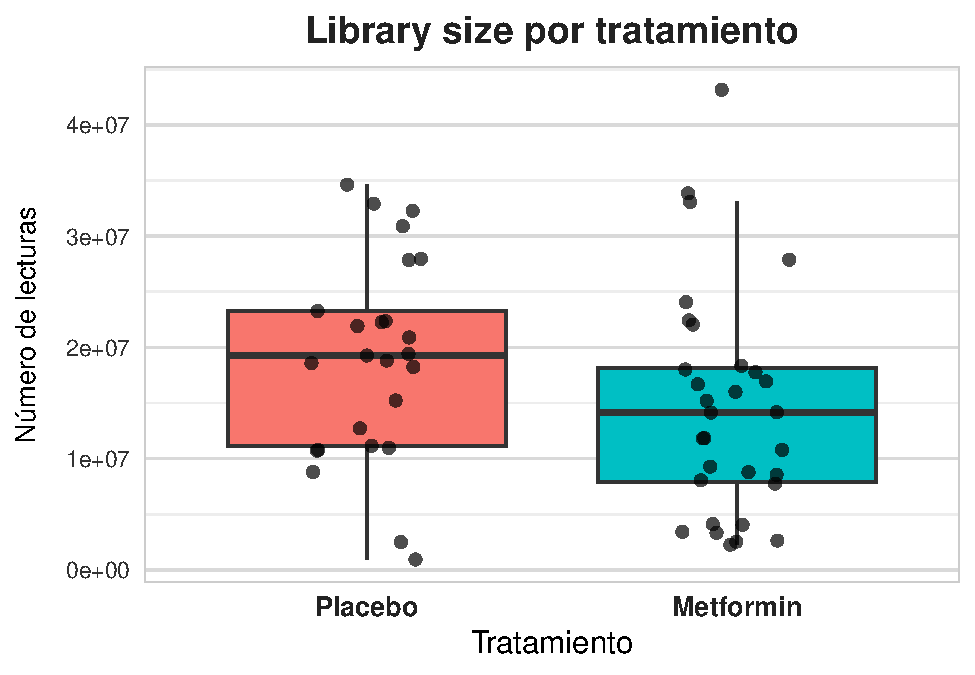
\includegraphics[keepaspectratio]{Proyecto_files/figure-latex/sequencing_depth-1.pdf}}

La mayoría de las muestras presentaron profundidades de secuenciación
dentro del rango esperado para estudios de RNA-seq en humanos (mediana ≈
16 millones de lecturas). Se identificó una muestra con un tamaño de
biblioteca considerablemente menor (\textasciitilde0.9 millones)
correspondiente a \texttt{Subject7}durante tratamiento placebo.

\subsubsection{Lecturas asignadas a
genes}\label{lecturas-asignadas-a-genes}

\begin{Shaded}
\begin{Highlighting}[]
\CommentTok{\# Calcular la proporción de lecturas asignadas a genes}
\NormalTok{rse\_muscle}\SpecialCharTok{$}\NormalTok{assigned\_gene\_prop }\OtherTok{\textless{}{-}}
\NormalTok{  rse\_muscle}\SpecialCharTok{$}\NormalTok{recount\_qc.gene\_fc\_count\_all.assigned }\SpecialCharTok{/}
\NormalTok{  rse\_muscle}\SpecialCharTok{$}\NormalTok{recount\_qc.gene\_fc\_count\_all.total}

\CommentTok{\# Resumen}
\FunctionTok{summary}\NormalTok{(rse\_muscle}\SpecialCharTok{$}\NormalTok{assigned\_gene\_prop)}
\end{Highlighting}
\end{Shaded}

\begin{verbatim}
##    Min. 1st Qu.  Median    Mean 3rd Qu.    Max. 
##  0.1004  0.5483  0.5582  0.5447  0.5684  0.5991
\end{verbatim}

\begin{Shaded}
\begin{Highlighting}[]
\CommentTok{\#Visualización}
\NormalTok{df\_qc }\OtherTok{\textless{}{-}} \FunctionTok{data.frame}\NormalTok{(}
  \AttributeTok{assigned\_gene\_prop =}\NormalTok{ rse\_muscle}\SpecialCharTok{$}\NormalTok{assigned\_gene\_prop}
\NormalTok{)}

\FunctionTok{ggplot}\NormalTok{(df\_qc, }\FunctionTok{aes}\NormalTok{(}\AttributeTok{x =}\NormalTok{ assigned\_gene\_prop)) }\SpecialCharTok{+}
  \FunctionTok{geom\_histogram}\NormalTok{(}\AttributeTok{bins =} \DecValTok{20}\NormalTok{, }\AttributeTok{color =} \StringTok{"black"}\NormalTok{, }\AttributeTok{fill =} \StringTok{"\#2C7FB8"}\NormalTok{) }\SpecialCharTok{+}
  \FunctionTok{theme\_bw}\NormalTok{() }\SpecialCharTok{+}
  \FunctionTok{labs}\NormalTok{(}
    \AttributeTok{title =} \StringTok{"Proporción de lecturas asignadas a genes"}\NormalTok{,}
    \AttributeTok{x =} \StringTok{"Fracción de lecturas"}\NormalTok{,}
    \AttributeTok{y =} \StringTok{"Número de muestras"}
\NormalTok{  )}
\end{Highlighting}
\end{Shaded}

\pandocbounded{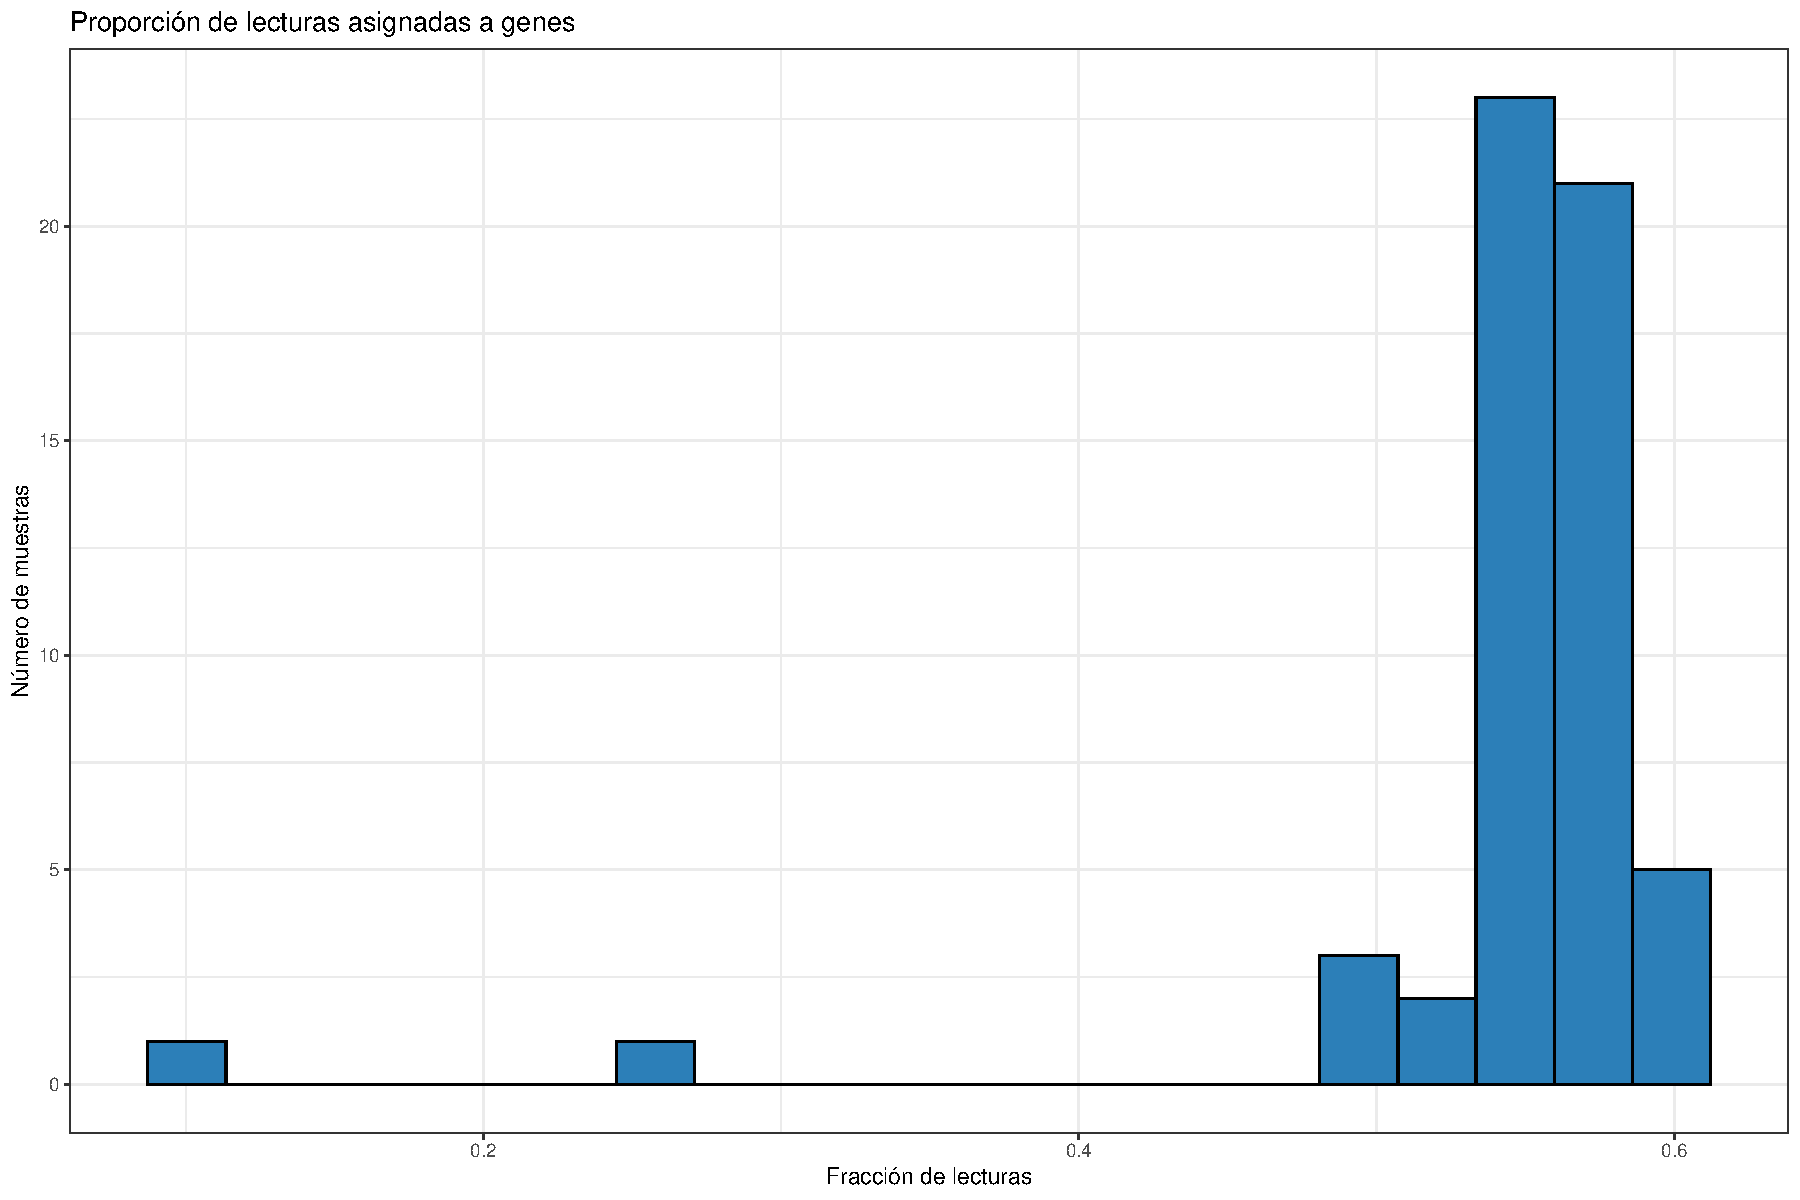
\includegraphics[keepaspectratio]{Proyecto_files/figure-latex/lectures_genes-1.pdf}}

\begin{Shaded}
\begin{Highlighting}[]
\CommentTok{\#Filtrar muestras con pocas lescturas asignadas}
\NormalTok{rse\_muscle\_filtered }\OtherTok{\textless{}{-}}\NormalTok{ rse\_muscle[,rse\_muscle}\SpecialCharTok{$}\NormalTok{assigned\_gene\_prop }\SpecialCharTok{\textgreater{}} \FloatTok{0.3}\NormalTok{]}

\CommentTok{\# Filtrar sujetos}
\NormalTok{tab }\OtherTok{\textless{}{-}} \FunctionTok{table}\NormalTok{(rse\_muscle\_filtered}\SpecialCharTok{$}\NormalTok{sra\_attribute.subject\_id,}
\NormalTok{             rse\_muscle\_filtered}\SpecialCharTok{$}\NormalTok{sra\_attribute.drug)}

\CommentTok{\# Sujetos con ambas condiciones}
\NormalTok{complete\_subjects }\OtherTok{\textless{}{-}} \FunctionTok{rownames}\NormalTok{(tab)[}\FunctionTok{rowSums}\NormalTok{(tab }\SpecialCharTok{\textgreater{}} \DecValTok{0}\NormalTok{) }\SpecialCharTok{==} \DecValTok{2}\NormalTok{]}

\NormalTok{rse\_muscle\_filtered }\OtherTok{\textless{}{-}}\NormalTok{ rse\_muscle\_filtered[,}
\NormalTok{  rse\_muscle\_filtered}\SpecialCharTok{$}\NormalTok{sra\_attribute.subject\_id }\SpecialCharTok{\%in\%}\NormalTok{ complete\_subjects}
\NormalTok{]}

\FunctionTok{kable}\NormalTok{(tab,}
      \AttributeTok{caption =} \StringTok{"Distribución de muestras por sujeto después del filtrado"}\NormalTok{)}
\end{Highlighting}
\end{Shaded}

\begin{longtable}[]{@{}lrr@{}}
\caption{Distribución de muestras por sujeto después del
filtrado}\tabularnewline
\toprule\noalign{}
& Placebo & Metformin \\
\midrule\noalign{}
\endfirsthead
\toprule\noalign{}
& Placebo & Metformin \\
\midrule\noalign{}
\endhead
\bottomrule\noalign{}
\endlastfoot
Subject1 & 2 & 1 \\
Subject10 & 2 & 2 \\
Subject11 & 2 & 4 \\
Subject12 & 4 & 4 \\
Subject13 & 2 & 4 \\
Subject14 & 2 & 0 \\
Subject2 & 1 & 2 \\
Subject3 & 2 & 2 \\
Subject4 & 2 & 1 \\
Subject5 & 1 & 0 \\
Subject6 & 1 & 3 \\
Subject7 & 2 & 4 \\
Subject9 & 2 & 2 \\
\end{longtable}

Se eliminaron los sujetos 5 y 14 debido a que tras el filtrado no
contaban con muestras en ambas condiciones.

\subsubsection{Filtrado de genes}\label{filtrado-de-genes}

\begin{Shaded}
\begin{Highlighting}[]
\CommentTok{\# Obtener counts}
\NormalTok{counts\_muscle\_filtered }\OtherTok{\textless{}{-}} \FunctionTok{assay}\NormalTok{(rse\_muscle\_filtered, }\StringTok{"counts"}\NormalTok{)}

\CommentTok{\# Crear DGEList primero}
\NormalTok{dge }\OtherTok{\textless{}{-}} \FunctionTok{DGEList}\NormalTok{(}\AttributeTok{counts =}\NormalTok{ counts\_muscle\_filtered, }\AttributeTok{genes =} \FunctionTok{rowData}\NormalTok{(rse\_muscle\_filtered))}

\CommentTok{\# Crear metadata correctamente}
\NormalTok{meta }\OtherTok{\textless{}{-}} \FunctionTok{data.frame}\NormalTok{(}
  \AttributeTok{group   =} \FunctionTok{factor}\NormalTok{(rse\_muscle\_filtered}\SpecialCharTok{$}\NormalTok{sra\_attribute.drug),}
  \AttributeTok{subject =} \FunctionTok{factor}\NormalTok{(rse\_muscle\_filtered}\SpecialCharTok{$}\NormalTok{sra\_attribute.subject\_id),}
  \AttributeTok{visit   =} \FunctionTok{factor}\NormalTok{(rse\_muscle\_filtered}\SpecialCharTok{$}\NormalTok{sra\_attribute.source\_name)}
\NormalTok{)}

\CommentTok{\# IMPORTANTE: rownames deben coincidir con columnas de counts}
\FunctionTok{rownames}\NormalTok{(meta) }\OtherTok{\textless{}{-}} \FunctionTok{colnames}\NormalTok{(dge)}

\CommentTok{\# Diseño para filtrado}
\NormalTok{design }\OtherTok{\textless{}{-}} \FunctionTok{model.matrix}\NormalTok{(}\SpecialCharTok{\textasciitilde{}}\NormalTok{ group, meta)}

\CommentTok{\# Filtrar genes}
\NormalTok{keep\_genes }\OtherTok{\textless{}{-}} \FunctionTok{filterByExpr}\NormalTok{(dge, }\AttributeTok{design =}\NormalTok{ design)}
\NormalTok{dge }\OtherTok{\textless{}{-}}\NormalTok{ dge[keep\_genes, , keep.lib.sizes }\OtherTok{=} \ConstantTok{FALSE}\NormalTok{]}

\CommentTok{\#Obtener nombres de genes filtrados}
\NormalTok{gene\_info }\OtherTok{\textless{}{-}} \FunctionTok{as.data.frame}\NormalTok{(}\FunctionTok{rowData}\NormalTok{(rse\_muscle\_filtered))}
\NormalTok{gene\_info\_filtered }\OtherTok{\textless{}{-}}\NormalTok{ gene\_info[keep\_genes, ]}

\NormalTok{dge}\SpecialCharTok{$}\NormalTok{genes }\OtherTok{\textless{}{-}} \FunctionTok{data.frame}\NormalTok{(}
  \AttributeTok{ENSEMBL =} \FunctionTok{rownames}\NormalTok{(dge),}
  \AttributeTok{SYMBOL  =}\NormalTok{ gene\_info\_filtered}\SpecialCharTok{$}\NormalTok{gene\_name}
\NormalTok{)}

\CommentTok{\# Número de genes filtrados}
\NormalTok{num\_genes\_retenidos }\OtherTok{\textless{}{-}} \FunctionTok{sum}\NormalTok{(keep\_genes)}
\NormalTok{num\_genes\_totales }\OtherTok{\textless{}{-}} \FunctionTok{nrow}\NormalTok{(counts\_muscle\_filtered)}

\CommentTok{\# Porcentaje de genes retenidos}
\NormalTok{porcentaje\_genes }\OtherTok{\textless{}{-}}\NormalTok{ (num\_genes\_retenidos }\SpecialCharTok{/}\NormalTok{ num\_genes\_totales) }\SpecialCharTok{*} \DecValTok{100}

\FunctionTok{cat}\NormalTok{(}\StringTok{"Genes retenidos:"}\NormalTok{, num\_genes\_retenidos, }\StringTok{"}\SpecialCharTok{\textbackslash{}n}\StringTok{"}\NormalTok{)}
\end{Highlighting}
\end{Shaded}

\begin{verbatim}
## Genes retenidos: 18509
\end{verbatim}

\begin{Shaded}
\begin{Highlighting}[]
\FunctionTok{cat}\NormalTok{(}\StringTok{"Total de genes:"}\NormalTok{, num\_genes\_totales, }\StringTok{"}\SpecialCharTok{\textbackslash{}n}\StringTok{"}\NormalTok{)}
\end{Highlighting}
\end{Shaded}

\begin{verbatim}
## Total de genes: 63856
\end{verbatim}

\begin{Shaded}
\begin{Highlighting}[]
\FunctionTok{cat}\NormalTok{(}\FunctionTok{sprintf}\NormalTok{(}\StringTok{"Porcentaje de genes retenidos: \%.2f\%\%}\SpecialCharTok{\textbackslash{}n}\StringTok{"}\NormalTok{, porcentaje\_genes))}
\end{Highlighting}
\end{Shaded}

\begin{verbatim}
## Porcentaje de genes retenidos: 28.99%
\end{verbatim}

\subsubsection{Exploración de
varianza}\label{exploraciuxf3n-de-varianza}

\begin{Shaded}
\begin{Highlighting}[]
\CommentTok{\# Asignar colores para cada grupo}

\NormalTok{colores }\OtherTok{\textless{}{-}} \FunctionTok{c}\NormalTok{(}\StringTok{"\#3dd0eeff"}\NormalTok{, }\StringTok{"\#FF7F7F"}\NormalTok{)}

\CommentTok{\#Plotear MDS con colores por grupo}
\FunctionTok{plotMDS}\NormalTok{(dge, }
        \AttributeTok{col =}\NormalTok{ colores[}\FunctionTok{as.numeric}\NormalTok{(meta}\SpecialCharTok{$}\NormalTok{group)],}
        \AttributeTok{pch =} \DecValTok{16}\NormalTok{,}
        \AttributeTok{cex =} \FloatTok{1.5}\NormalTok{,}
        \AttributeTok{main =} \StringTok{"MDS por tratamiento"}\NormalTok{,}
        \AttributeTok{xlab =} \StringTok{"Dimensión 1"}\NormalTok{,}
        \AttributeTok{ylab =} \StringTok{"Dimensión 2"}\NormalTok{)}

\CommentTok{\# Añadir leyenda }
\FunctionTok{legend}\NormalTok{(}\StringTok{"topright"}\NormalTok{, }
       \AttributeTok{legend =} \FunctionTok{levels}\NormalTok{(meta}\SpecialCharTok{$}\NormalTok{group),}
       \AttributeTok{col =}\NormalTok{ colores[}\DecValTok{1}\SpecialCharTok{:}\FunctionTok{length}\NormalTok{(}\FunctionTok{levels}\NormalTok{(meta}\SpecialCharTok{$}\NormalTok{group))], }
       \AttributeTok{pch =} \DecValTok{16}\NormalTok{,}
       \AttributeTok{cex =} \FloatTok{0.8}\NormalTok{,}
       \AttributeTok{title =} \StringTok{"Tratamiento"}\NormalTok{,}
       \AttributeTok{bty =} \StringTok{"o"}\NormalTok{,           }
       \AttributeTok{bg =} \StringTok{"white"}\NormalTok{,        }
       \AttributeTok{box.lwd =} \DecValTok{1}\NormalTok{)         }
\end{Highlighting}
\end{Shaded}

\pandocbounded{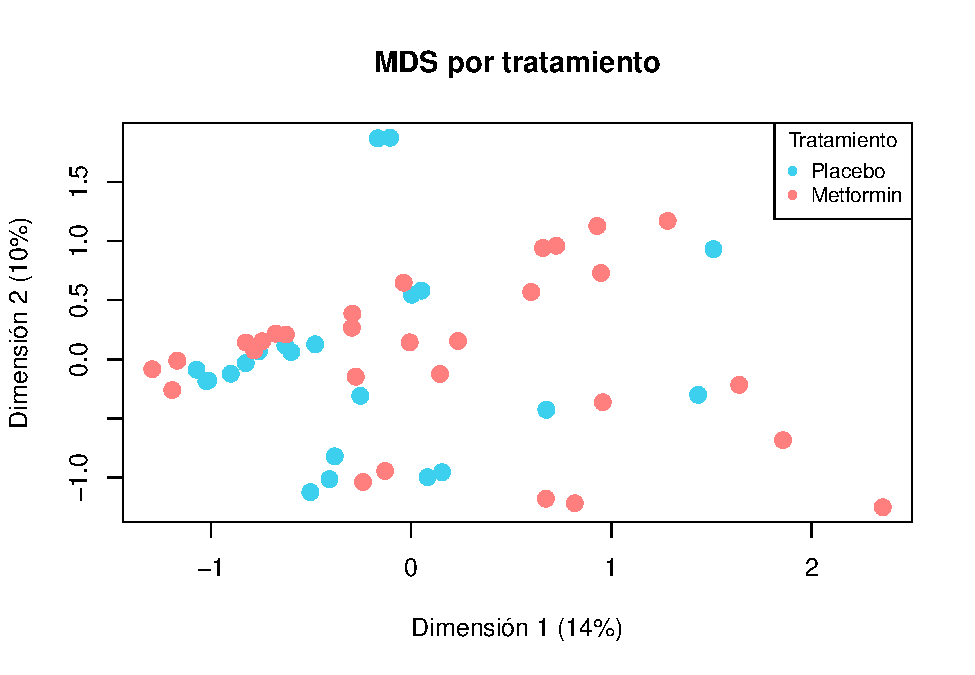
\includegraphics[keepaspectratio]{Proyecto_files/figure-latex/MDS-1.pdf}}

El análisis de escalamiento multidimensional (MDS) no mostró una
separación evidente entre las condiciones de metformina y placebo en los
primeros componentes principales. Dado que el MDS sugiere la presencia
de múltiples fuentes de variabilidad en los datos, se procedió a
realizar un análisis de partición de varianza mediante modelos lineales
mixtos para cuantificar formalmente la contribución relativa del sujeto
y del tratamiento a la variación transcriptómica observada.

\begin{Shaded}
\begin{Highlighting}[]
\NormalTok{form\_vp }\OtherTok{\textless{}{-}} \ErrorTok{\textasciitilde{}}\NormalTok{ (}\DecValTok{1}\SpecialCharTok{|}\NormalTok{group) }\SpecialCharTok{+}\NormalTok{ (}\DecValTok{1}\SpecialCharTok{|}\NormalTok{subject) }\SpecialCharTok{+}\NormalTok{ (}\DecValTok{1}\SpecialCharTok{|}\NormalTok{visit)}
\NormalTok{param }\OtherTok{\textless{}{-}} \FunctionTok{SerialParam}\NormalTok{(}\AttributeTok{progressbar =} \ConstantTok{TRUE}\NormalTok{)}
\NormalTok{vobj }\OtherTok{\textless{}{-}} \FunctionTok{voomWithDreamWeights}\NormalTok{(dge, form\_vp, meta, }\AttributeTok{BPPARAM =}\NormalTok{ param)}
\NormalTok{vp }\OtherTok{\textless{}{-}} \FunctionTok{fitExtractVarPartModel}\NormalTok{(vobj, form\_vp, meta, }\AttributeTok{BPPARAM =}\NormalTok{ param)}
\FunctionTok{plotVarPart}\NormalTok{(vp)}
\end{Highlighting}
\end{Shaded}

\pandocbounded{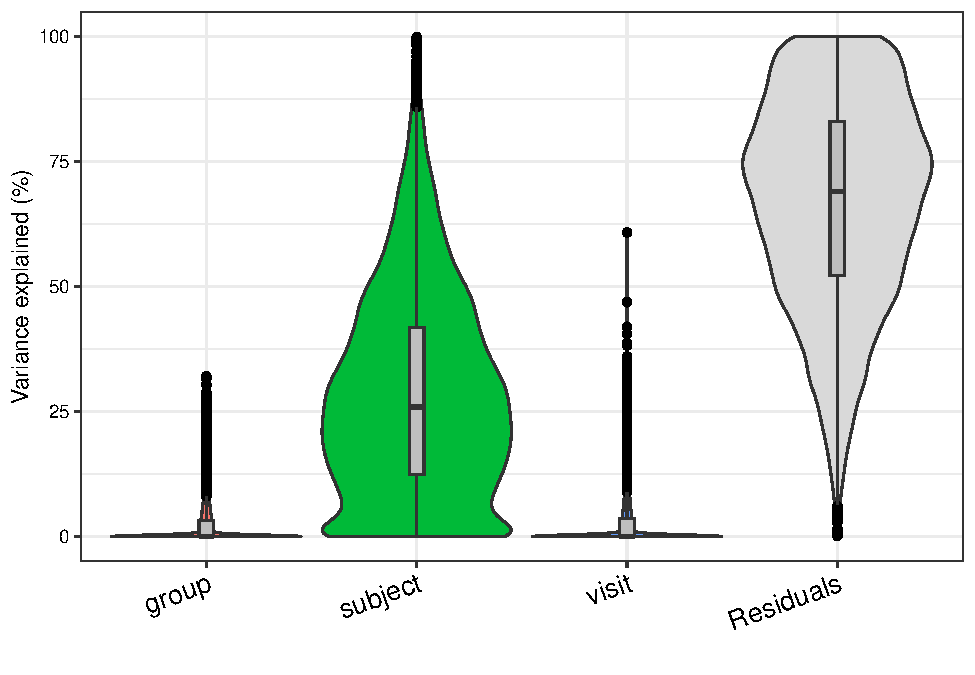
\includegraphics[keepaspectratio]{Proyecto_files/figure-latex/variance_partition-1.pdf}}

Para evaluar la contribución de las variables experimentales a la
varianza global de los datos de expresión génica, se realizó un análisis
de partición de la varianza. El factor `subject' (sujeto) emergió como
una fuente significativa de variación, explicando una proporción
sustancial de la varianza en un gran número de genes, lo que justifica
su inclusión en el modelo lineal para controlar la heterogeneidad
interindividual. Por el contrario, las variables `group' (grupo) y
`visit' (visita) mostraron una contribución marginal a la varianza total
en la mayoría de los genes. Cabe destacar que se observó una fracción
elevada de varianza residual, lo que sugiere la presencia de ruido
técnico o biológico no capturado por el diseño inicial, subrayando la
importancia de emplear métodos robustos de normalización y filtrado
antes del análisis de expresión diferencial

\subsubsection{Análisis de expresión
diferencial}\label{anuxe1lisis-de-expresiuxf3n-diferencial}

\begin{Shaded}
\begin{Highlighting}[]
\CommentTok{\# Analisis de expresión diferencial con dream}
\NormalTok{form\_de }\OtherTok{\textless{}{-}} \ErrorTok{\textasciitilde{}}\NormalTok{ group }\SpecialCharTok{+}\NormalTok{ (}\DecValTok{1}\SpecialCharTok{|}\NormalTok{subject)}
\NormalTok{param }\OtherTok{\textless{}{-}} \FunctionTok{SerialParam}\NormalTok{(}\AttributeTok{progressbar =} \ConstantTok{TRUE}\NormalTok{)}
\NormalTok{vobj\_de }\OtherTok{\textless{}{-}} \FunctionTok{voomWithDreamWeights}\NormalTok{(dge, form\_de, meta, }\AttributeTok{BPPARAM =}\NormalTok{ param, }\AttributeTok{plot=}\ConstantTok{TRUE}\NormalTok{)}
\end{Highlighting}
\end{Shaded}

\pandocbounded{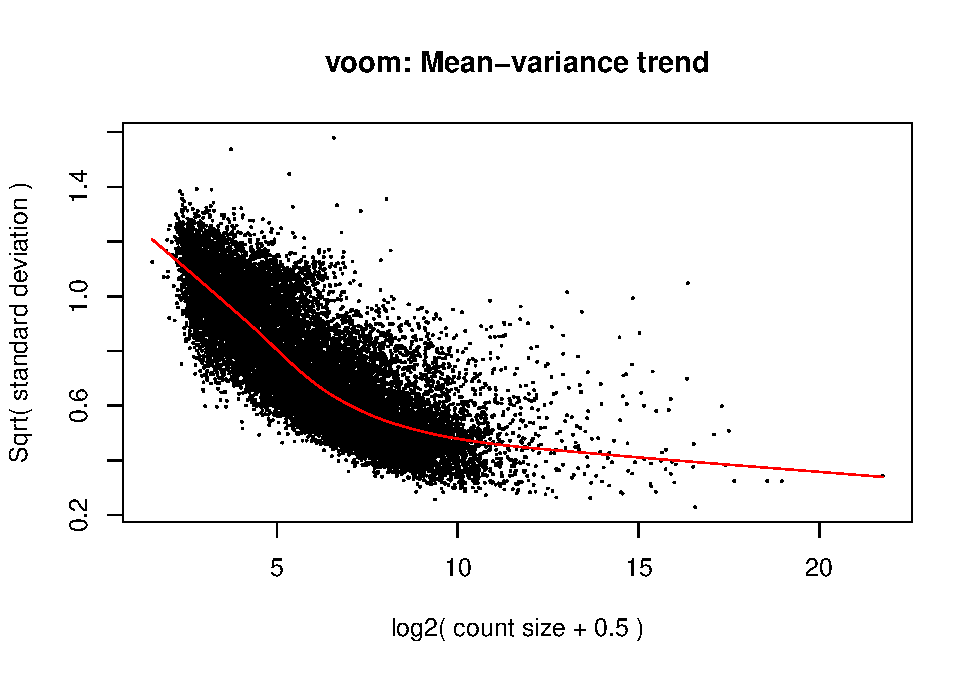
\includegraphics[keepaspectratio]{Proyecto_files/figure-latex/differential_expression-1.pdf}}

\begin{Shaded}
\begin{Highlighting}[]
\NormalTok{fit }\OtherTok{\textless{}{-}} \FunctionTok{dream}\NormalTok{(vobj\_de, form\_de, meta, }\AttributeTok{BPPARAM =}\NormalTok{ param)}
\NormalTok{fit }\OtherTok{\textless{}{-}} \FunctionTok{eBayes}\NormalTok{(fit)}
\NormalTok{res }\OtherTok{\textless{}{-}} \FunctionTok{topTable}\NormalTok{(fit, }\AttributeTok{coef =} \StringTok{"groupMetformin"}\NormalTok{, }\AttributeTok{number =} \ConstantTok{Inf}\NormalTok{, }\AttributeTok{sort.by =} \StringTok{"P"}\NormalTok{)}
\FunctionTok{head}\NormalTok{(res)}
\end{Highlighting}
\end{Shaded}

\begin{verbatim}
##                               ENSEMBL       SYMBOL      logFC  AveExpr
## ENSG00000268518.1   ENSG00000268518.1 CTD-2545M3.8 -0.4988174 4.946287
## ENSG00000267165.1   ENSG00000267165.1   CHMP1B-AS1  0.5091815 2.934566
## ENSG00000255112.2   ENSG00000255112.2       CHMP1B  0.3596053 4.807522
## ENSG00000004799.7   ENSG00000004799.7         PDK4  1.0857437 8.627689
## ENSG00000273540.3   ENSG00000273540.3        AGBL1 -0.3055320 5.210083
## ENSG00000170310.14 ENSG00000170310.14         STX8  0.4798080 2.582933
##                            t      P.Value    adj.P.Val        B     z.std
## ENSG00000268518.1  -6.924079 1.969431e-08 0.0002634524 8.957820 -5.614665
## ENSG00000267165.1   6.708402 3.953982e-08 0.0002634524 8.317751  5.492895
## ENSG00000255112.2   6.695653 4.270124e-08 0.0002634524 8.252060  5.479300
## ENSG00000004799.7   6.456141 8.700241e-08 0.0004025819 7.565032  5.351969
## ENSG00000273540.3  -6.183153 2.365291e-07 0.0008755836 6.748522 -5.168066
## ENSG00000170310.14  5.773738 8.819095e-07 0.0027205437 5.607397  4.916309
\end{verbatim}

\paragraph{MA plot}\label{ma-plot}

\begin{Shaded}
\begin{Highlighting}[]
\NormalTok{df }\OtherTok{\textless{}{-}} \FunctionTok{data.frame}\NormalTok{(}
  \AttributeTok{AveExpr =}\NormalTok{ res}\SpecialCharTok{$}\NormalTok{AveExpr,}
  \AttributeTok{logFC =}\NormalTok{ res}\SpecialCharTok{$}\NormalTok{logFC,}
  \AttributeTok{P =}\NormalTok{ res}\SpecialCharTok{$}\NormalTok{P.Value,}
  \AttributeTok{FDR =}\NormalTok{ res}\SpecialCharTok{$}\NormalTok{adj.P.Val}
\NormalTok{)}

\NormalTok{df}\SpecialCharTok{$}\NormalTok{Significant }\OtherTok{\textless{}{-}}\NormalTok{ df}\SpecialCharTok{$}\NormalTok{FDR }\SpecialCharTok{\textless{}} \FloatTok{0.05}

\FunctionTok{ggplot}\NormalTok{(df, }\FunctionTok{aes}\NormalTok{(AveExpr, logFC)) }\SpecialCharTok{+}
  
  \CommentTok{\# No significativos}
  \FunctionTok{geom\_point}\NormalTok{(}\AttributeTok{data =} \FunctionTok{subset}\NormalTok{(df, Significant }\SpecialCharTok{==} \ConstantTok{FALSE}\NormalTok{),}
             \AttributeTok{color =} \StringTok{"grey75"}\NormalTok{,}
             \AttributeTok{alpha =} \FloatTok{0.5}\NormalTok{,}
             \AttributeTok{size =} \DecValTok{1}\NormalTok{) }\SpecialCharTok{+}
  
  \CommentTok{\# Significativos encima}
  \FunctionTok{geom\_point}\NormalTok{(}\AttributeTok{data =} \FunctionTok{subset}\NormalTok{(df, Significant }\SpecialCharTok{==} \ConstantTok{TRUE}\NormalTok{),}
             \AttributeTok{color =} \StringTok{"\#ff3c3cff"}\NormalTok{, }
             \AttributeTok{alpha =} \FloatTok{0.9}\NormalTok{,}
             \AttributeTok{size =} \FloatTok{1.3}\NormalTok{) }\SpecialCharTok{+}
  
  \CommentTok{\# Línea central}
  \FunctionTok{geom\_hline}\NormalTok{(}\AttributeTok{yintercept =} \DecValTok{0}\NormalTok{,}
             \AttributeTok{color =} \StringTok{"black"}\NormalTok{,}
             \AttributeTok{linewidth =} \FloatTok{0.6}\NormalTok{) }\SpecialCharTok{+}
  
  \CommentTok{\# Umbral biológico ±1}
  \FunctionTok{geom\_hline}\NormalTok{(}\AttributeTok{yintercept =} \FunctionTok{c}\NormalTok{(}\SpecialCharTok{{-}}\DecValTok{1}\NormalTok{,}\DecValTok{1}\NormalTok{),}
             \AttributeTok{linetype =} \StringTok{"dashed"}\NormalTok{,}
             \AttributeTok{color =} \StringTok{"black"}\NormalTok{,}
             \AttributeTok{linewidth =} \FloatTok{0.4}\NormalTok{) }\SpecialCharTok{+}
  
  \FunctionTok{theme\_classic}\NormalTok{(}\AttributeTok{base\_size =} \DecValTok{14}\NormalTok{) }\SpecialCharTok{+}
  \FunctionTok{labs}\NormalTok{(}\AttributeTok{title =} \StringTok{"MA Plot: Metformin vs Placebo"}\NormalTok{,}
       \AttributeTok{x =} \StringTok{"Average log{-}expression"}\NormalTok{,}
       \AttributeTok{y =} \StringTok{"Log2 Fold Change"}\NormalTok{) }\SpecialCharTok{+}
  \FunctionTok{theme}\NormalTok{(}\AttributeTok{legend.position =} \StringTok{"none"}\NormalTok{)}
\end{Highlighting}
\end{Shaded}

\pandocbounded{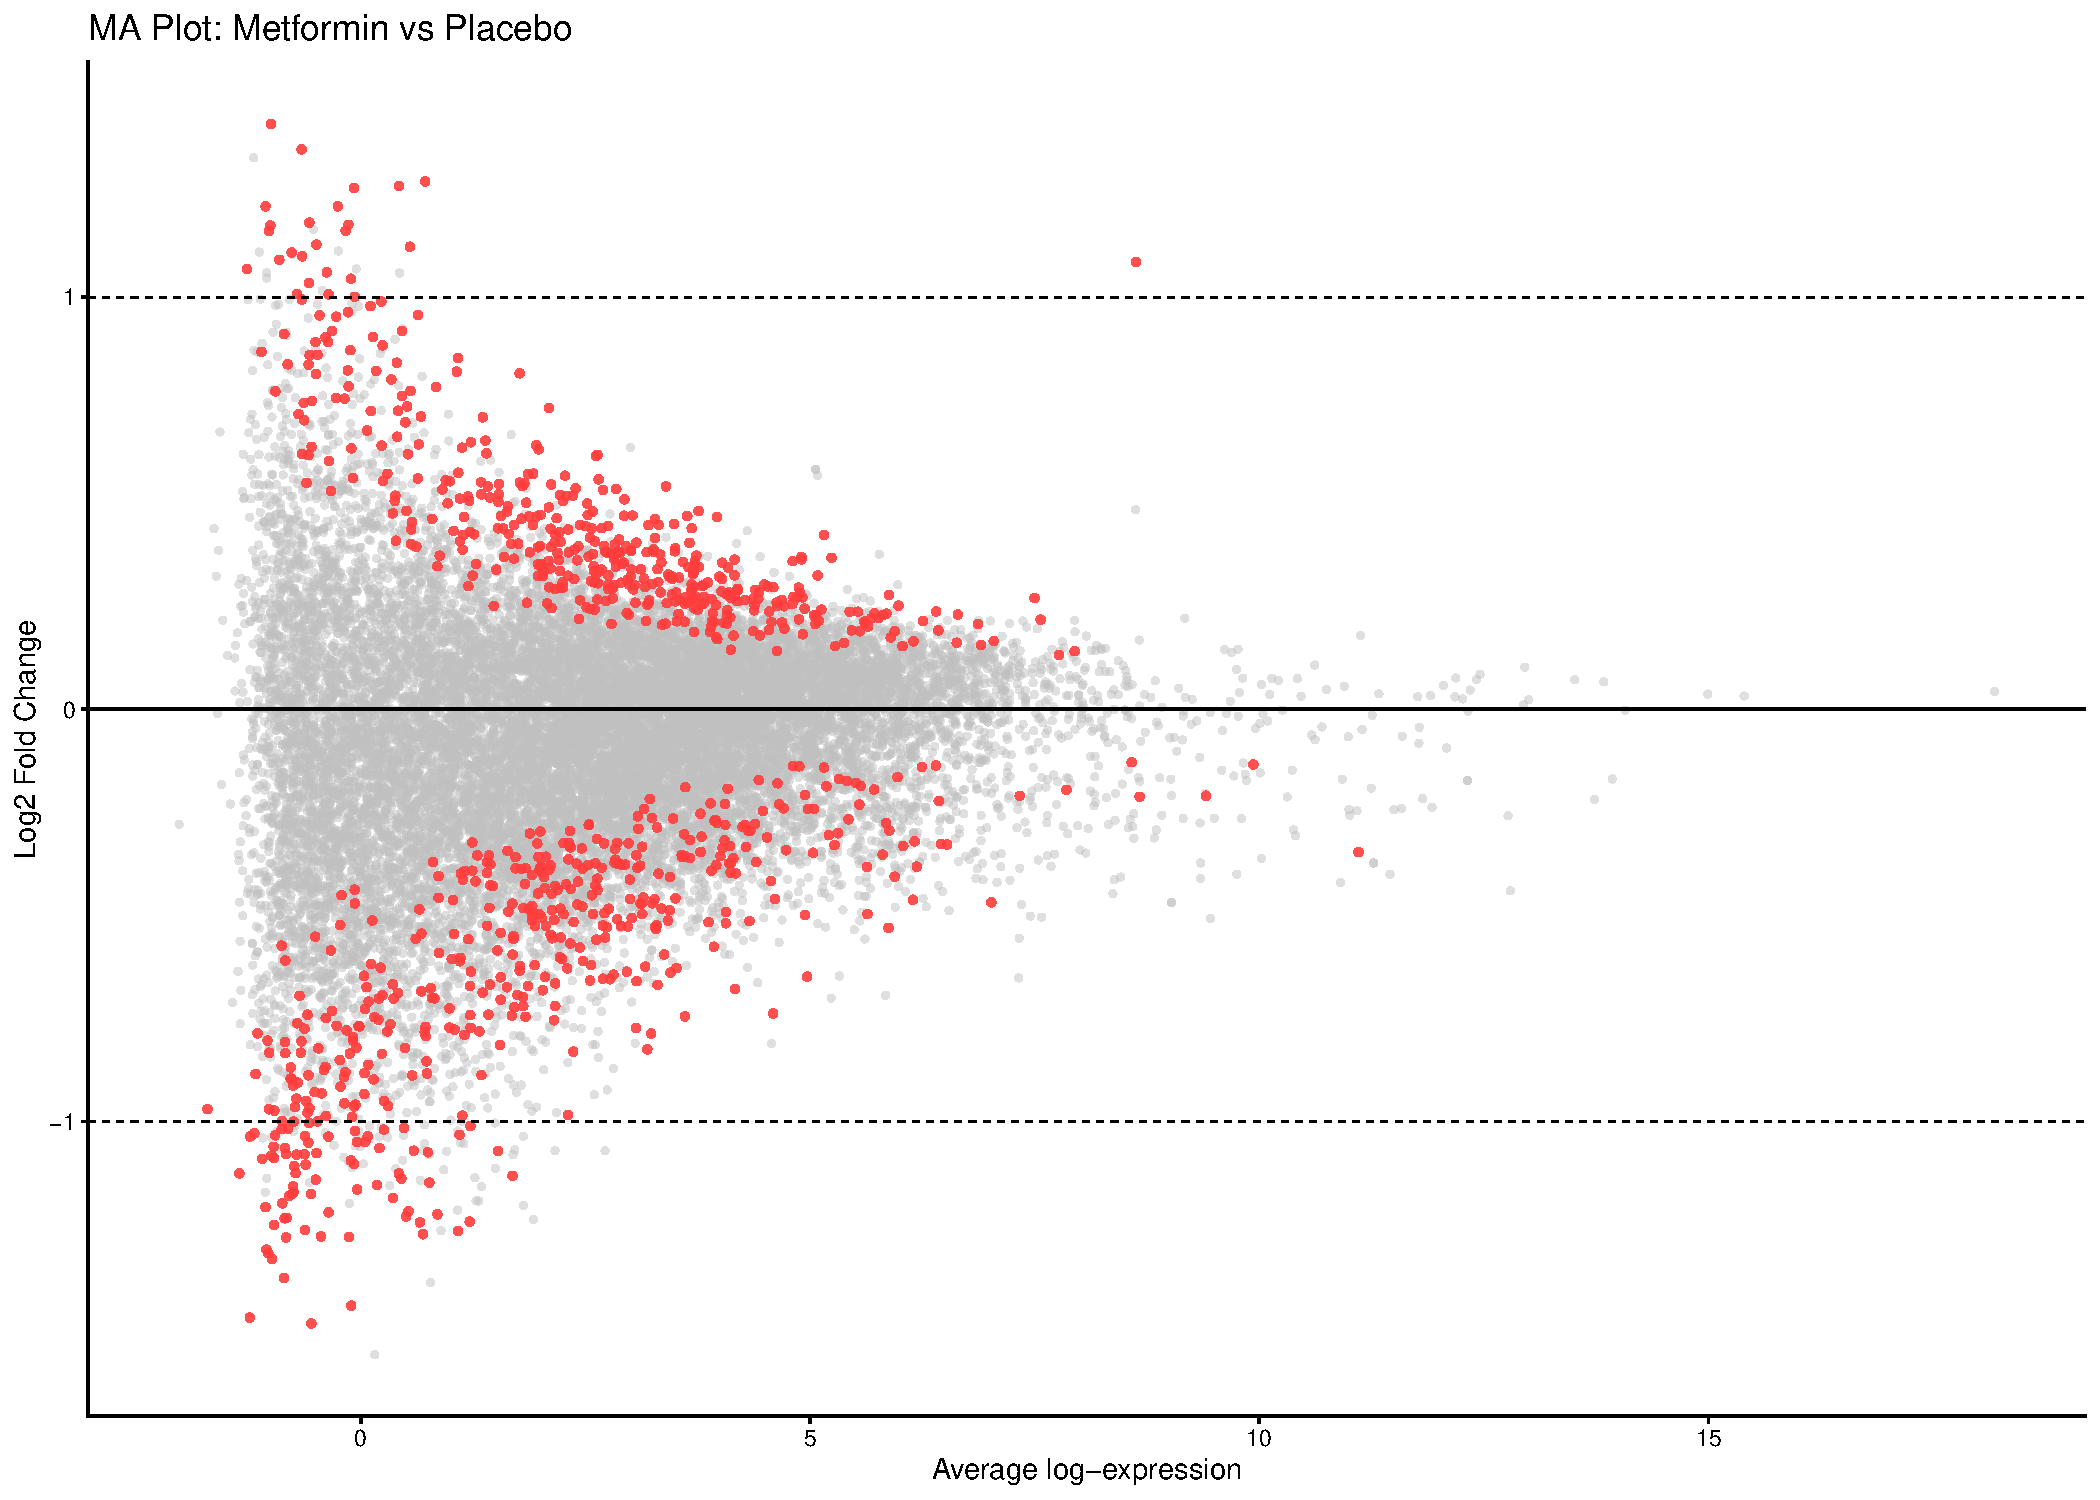
\includegraphics[keepaspectratio]{Proyecto_files/figure-latex/MA_plot-1.pdf}}

En el MA plot se observa que la mayoría de los genes significativamente
expresados (FDR \textless{} 0.05) presentan cambios moderados en la
expresión (logFC entre -1 y 1). Esto sugiere que, aunque existen
diferencias estadísticamente significativas, la respuesta al tratamiento
con metformina en músculo esquelético no es masiva, sino que se
manifiesta como ajustes finos y moderados en la expresión génica.

Además, se aprecia una alta densidad de genes significativos en el rango
de baja expresión (lado izquierdo del gráfico). La distribución
simétrica de genes regulados positivamente y negativamente indica un
impacto equilibrado sobre la homeostasis celular del músculo
esquelético. Cabe destacar que se identificaron DEGs a lo largo de un
amplio espectro de niveles de abundancia, lo que subraya la eficacia del
filtrado y la normalización empleados para detectar cambios sutiles pero
consistentes estadísticamente.

Dado que se trata de la respuesta a un tratamiento y considerando la
variabilidad individual observada, los genes regulados positiva y
negativamente (UP y DOWN) se consideraron con un umbral más bajo de
logFC ≥ 0.5, siguiendo la misma estrategia aplicada en el artículo de
referencia

\begin{Shaded}
\begin{Highlighting}[]
\CommentTok{\# Volcanoplot}

\NormalTok{res}\SpecialCharTok{$}\NormalTok{Category }\OtherTok{\textless{}{-}} \StringTok{"NS"}

\CommentTok{\# Primero los verdaderamente DE}
\NormalTok{res}\SpecialCharTok{$}\NormalTok{Category[res}\SpecialCharTok{$}\NormalTok{logFC }\SpecialCharTok{\textgreater{}} \FloatTok{0.5} \SpecialCharTok{\&}\NormalTok{ res}\SpecialCharTok{$}\NormalTok{adj.P.Val }\SpecialCharTok{\textless{}} \FloatTok{0.05}\NormalTok{] }\OtherTok{\textless{}{-}} \StringTok{"UP"}
\NormalTok{res}\SpecialCharTok{$}\NormalTok{Category[res}\SpecialCharTok{$}\NormalTok{logFC }\SpecialCharTok{\textless{}} \SpecialCharTok{{-}}\FloatTok{0.5} \SpecialCharTok{\&}\NormalTok{ res}\SpecialCharTok{$}\NormalTok{adj.P.Val }\SpecialCharTok{\textless{}} \FloatTok{0.05}\NormalTok{] }\OtherTok{\textless{}{-}} \StringTok{"DOWN"}

\CommentTok{\# Luego los parciales}
\NormalTok{res}\SpecialCharTok{$}\NormalTok{Category[}\FunctionTok{abs}\NormalTok{(res}\SpecialCharTok{$}\NormalTok{logFC) }\SpecialCharTok{\textgreater{}} \FloatTok{0.5} \SpecialCharTok{\&}\NormalTok{ res}\SpecialCharTok{$}\NormalTok{adj.P.Val }\SpecialCharTok{\textgreater{}=} \FloatTok{0.05}\NormalTok{] }\OtherTok{\textless{}{-}} \StringTok{"logFC"}
\NormalTok{res}\SpecialCharTok{$}\NormalTok{Category[}\FunctionTok{abs}\NormalTok{(res}\SpecialCharTok{$}\NormalTok{logFC) }\SpecialCharTok{\textless{}=} \FloatTok{0.5} \SpecialCharTok{\&}\NormalTok{ res}\SpecialCharTok{$}\NormalTok{adj.P.Val }\SpecialCharTok{\textless{}} \FloatTok{0.05}\NormalTok{] }\OtherTok{\textless{}{-}} \StringTok{"p{-}value"}

\CommentTok{\# colores}
\NormalTok{keyvals }\OtherTok{\textless{}{-}} \FunctionTok{c}\NormalTok{(}
  \AttributeTok{NS =} \StringTok{"grey85"}\NormalTok{,}
  \AttributeTok{logFC =} \StringTok{"\#e0d688ff"}\NormalTok{,}
  \StringTok{\textasciigrave{}}\AttributeTok{p{-}value}\StringTok{\textasciigrave{}} \OtherTok{=} \StringTok{"\#a186c4ff"}\NormalTok{,}
  \AttributeTok{UP =} \StringTok{"\#FF7F7F"}\NormalTok{,}
  \AttributeTok{DOWN =} \StringTok{"\#3dd0eeff"}
\NormalTok{)}

\NormalTok{colCustom }\OtherTok{\textless{}{-}}\NormalTok{ keyvals[res}\SpecialCharTok{$}\NormalTok{Category]}


\CommentTok{\# Volcano plot con EnhancedVolcano}
\FunctionTok{EnhancedVolcano}\NormalTok{(}
\NormalTok{  res,}
  \AttributeTok{lab =} \FunctionTok{ifelse}\NormalTok{(}\FunctionTok{is.na}\NormalTok{(res}\SpecialCharTok{$}\NormalTok{SYMBOL) }\SpecialCharTok{|}\NormalTok{ res}\SpecialCharTok{$}\NormalTok{SYMBOL }\SpecialCharTok{==} \StringTok{""}\NormalTok{, }\FunctionTok{rownames}\NormalTok{(res), res}\SpecialCharTok{$}\NormalTok{SYMBOL),}
  \AttributeTok{x =} \StringTok{"logFC"}\NormalTok{,}
  \AttributeTok{y =} \StringTok{"adj.P.Val"}\NormalTok{,}
  \AttributeTok{xlim =} \FunctionTok{c}\NormalTok{(}\SpecialCharTok{{-}}\DecValTok{2}\NormalTok{, }\DecValTok{2}\NormalTok{),}
  \AttributeTok{ylim =} \FunctionTok{c}\NormalTok{(}\DecValTok{0}\NormalTok{, }\FloatTok{5.5}\NormalTok{),}
  \AttributeTok{ylab =} \FunctionTok{expression}\NormalTok{(}\SpecialCharTok{{-}}\NormalTok{Log[}\DecValTok{10}\NormalTok{]}\SpecialCharTok{\textasciitilde{}}\NormalTok{adj}\SpecialCharTok{\textasciitilde{}}\NormalTok{P),}
  \AttributeTok{pCutoff =} \FloatTok{0.05}\NormalTok{,}
  \AttributeTok{FCcutoff =} \FloatTok{0.5}\NormalTok{,}
  \AttributeTok{selectLab =} \FunctionTok{c}\NormalTok{(}\StringTok{"PDK4"}\NormalTok{, }\StringTok{"TAS2R46"}\NormalTok{, }\StringTok{"SLC1A1"}\NormalTok{, }\StringTok{"HLA{-}DOA"}\NormalTok{, }\StringTok{"HOXD4"}\NormalTok{, }\StringTok{"BEX4"}\NormalTok{, }\StringTok{"CCL5"}\NormalTok{, }\StringTok{"RNF43"}\NormalTok{, }\StringTok{"GAPDHP42"}\NormalTok{, }\StringTok{"HRASLS5"}\NormalTok{, }\StringTok{"PPARGC1A"}\NormalTok{, }\StringTok{"SLC2A4"}\NormalTok{, }\StringTok{"PCK1"}\NormalTok{, }\StringTok{"RET"}\NormalTok{, }\StringTok{"RBBP8"}\NormalTok{, }\StringTok{"RPS6KA6"}\NormalTok{, }\StringTok{"ANGPT2"}\NormalTok{, }\StringTok{"SLC38A9"}\NormalTok{, }\StringTok{"GRAMD1B"}\NormalTok{, }\StringTok{"THBD"}\NormalTok{, }\StringTok{"RARRES3"}\NormalTok{, }\StringTok{"AFMID"}\NormalTok{),}
  \AttributeTok{xlab =} \FunctionTok{bquote}\NormalTok{(}\SpecialCharTok{\textasciitilde{}}\NormalTok{Log[}\DecValTok{2}\NormalTok{]}\SpecialCharTok{\textasciitilde{}} \StringTok{\textquotesingle{}fold change\textquotesingle{}}\NormalTok{),}
  \AttributeTok{labSize =} \FloatTok{3.5}\NormalTok{,}
  \AttributeTok{labCol =} \StringTok{"black"}\NormalTok{,}
  \AttributeTok{labFace =} \StringTok{"bold"}\NormalTok{,}
  \AttributeTok{boxedLabels =} \ConstantTok{TRUE}\NormalTok{,}
  \AttributeTok{drawConnectors =} \ConstantTok{TRUE}\NormalTok{,}
  \AttributeTok{widthConnectors =} \FloatTok{0.5}\NormalTok{,}
  \AttributeTok{colConnectors =} \StringTok{"black"}\NormalTok{,}
  \AttributeTok{cutoffLineType =} \StringTok{"twodash"}\NormalTok{,}
  \AttributeTok{pointSize =} \FloatTok{2.5}\NormalTok{,}
  \AttributeTok{colCustom =}\NormalTok{ colCustom,}
  \AttributeTok{cutoffLineWidth =} \FloatTok{0.8}\NormalTok{,}
  \AttributeTok{title =} \StringTok{"Metformin vs Placebo"}\NormalTok{,}
  \AttributeTok{subtitle =} \StringTok{"Expresión diferencial en músculo esquelético"}\NormalTok{,}
  \AttributeTok{caption =} \FunctionTok{paste0}\NormalTok{(}\FunctionTok{sum}\NormalTok{(res}\SpecialCharTok{$}\NormalTok{Category }\SpecialCharTok{==} \StringTok{"UP"}\NormalTok{), }\StringTok{" upregulated; "}\NormalTok{,}
                   \FunctionTok{sum}\NormalTok{(res}\SpecialCharTok{$}\NormalTok{Category }\SpecialCharTok{==} \StringTok{"DOWN"}\NormalTok{), }\StringTok{" downregulated"}\NormalTok{)}
\NormalTok{)}
\end{Highlighting}
\end{Shaded}

\pandocbounded{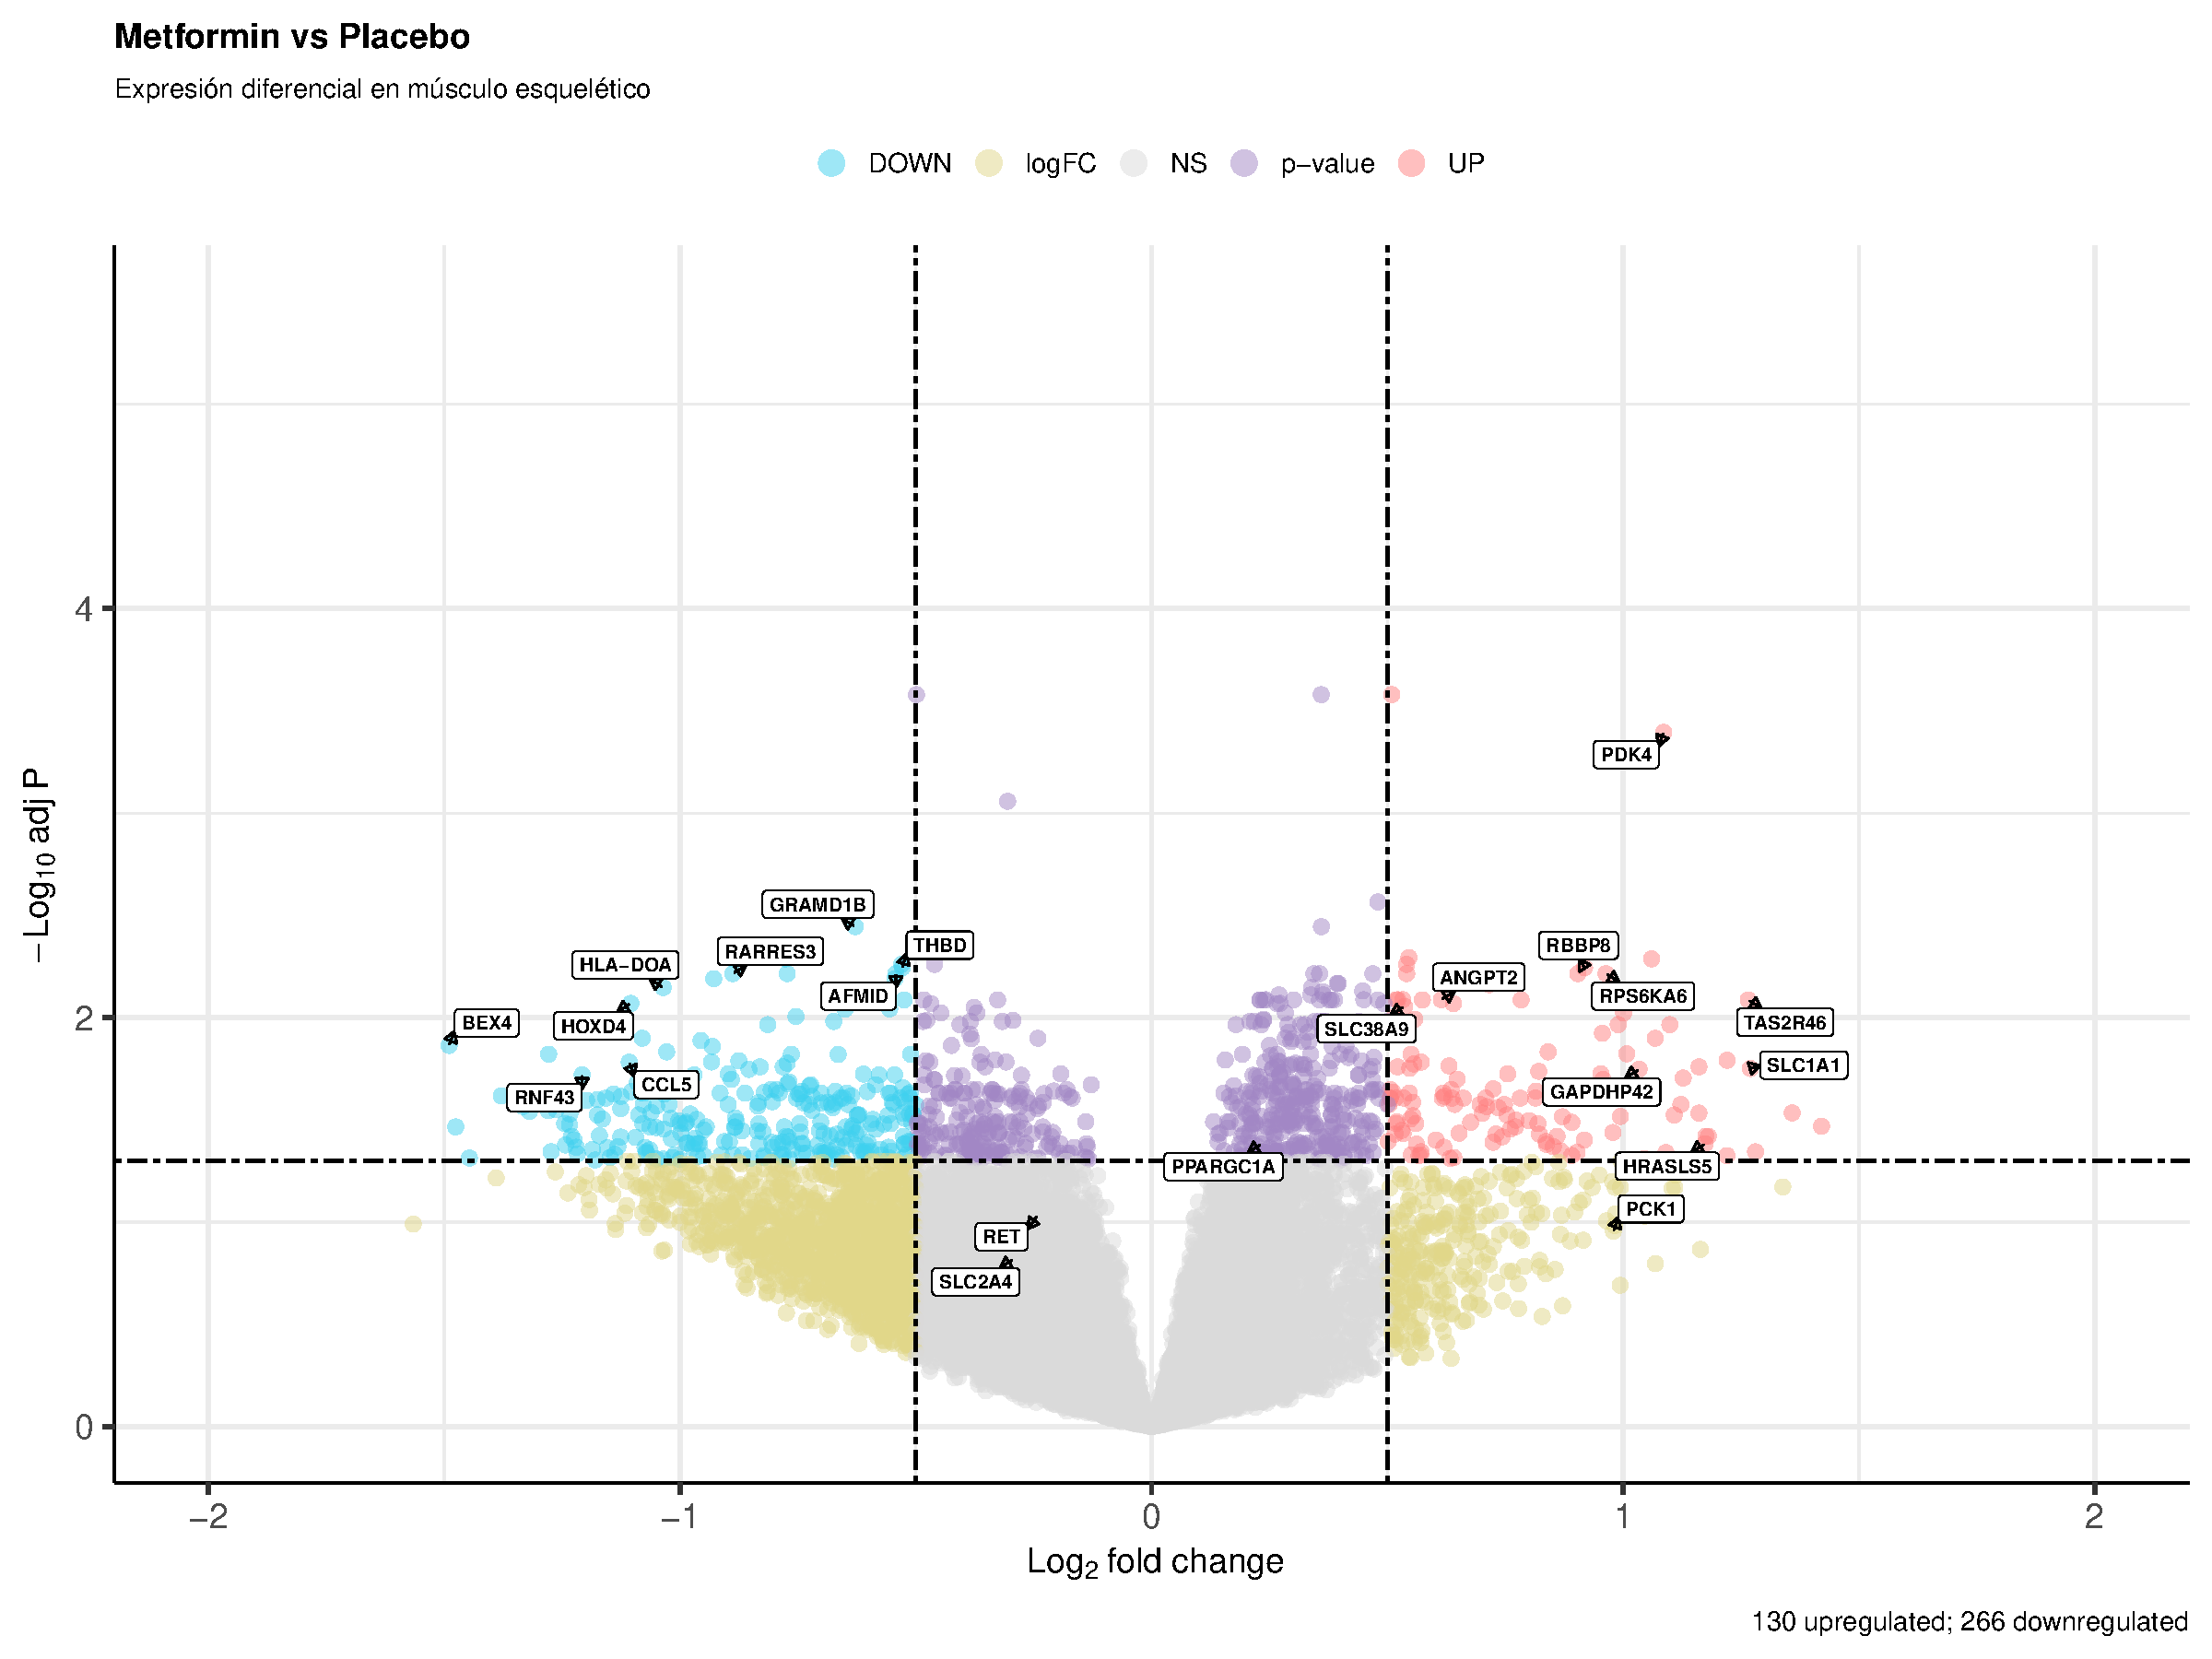
\includegraphics[keepaspectratio]{Proyecto_files/figure-latex/Volcano_plot-1.pdf}}

\begin{Shaded}
\begin{Highlighting}[]
\CommentTok{\# Guardar resultados }
\NormalTok{UP\_genes   }\OtherTok{\textless{}{-}}\NormalTok{ res[res}\SpecialCharTok{$}\NormalTok{Category }\SpecialCharTok{==} \StringTok{"UP"}\NormalTok{, ]}
\NormalTok{DOWN\_genes }\OtherTok{\textless{}{-}}\NormalTok{ res[res}\SpecialCharTok{$}\NormalTok{Category }\SpecialCharTok{==} \StringTok{"DOWN"}\NormalTok{, ]}
\NormalTok{FDR\_only }\OtherTok{\textless{}{-}}\NormalTok{ res[res}\SpecialCharTok{$}\NormalTok{Category }\SpecialCharTok{==} \StringTok{"p{-}value"}\NormalTok{, ]}

\FunctionTok{nrow}\NormalTok{(UP\_genes)}
\end{Highlighting}
\end{Shaded}

\begin{verbatim}
## [1] 130
\end{verbatim}

\begin{Shaded}
\begin{Highlighting}[]
\FunctionTok{nrow}\NormalTok{(DOWN\_genes)}
\end{Highlighting}
\end{Shaded}

\begin{verbatim}
## [1] 266
\end{verbatim}

\begin{Shaded}
\begin{Highlighting}[]
\FunctionTok{nrow}\NormalTok{(FDR\_only)}
\end{Highlighting}
\end{Shaded}

\begin{verbatim}
## [1] 525
\end{verbatim}

El análisis de expresión diferencial, visualizado mediante un Volcano
Plot, identificó un total de 396 genes significativamente regulados por
la metformina bajo un umbral de \(|Log_2FC| > 0.5\) y \(FDR < 0.05\)
(130 incrementados y 266 disminuidos). Además, se identificaron 525
genes adicionales que alcanzaron significancia estadística
(\(FDR < 0.05\)) con magnitudes de cambio menores, sugiriendo una
modulación transcriptómica extensa pero sutil. Entre los genes con mayor
significancia y magnitud destacan PDK4, SLC1A1, CCL5 y HLA-DOA. La
robustez de estos hallazgos, a pesar de la heterogeneidad
interindividual, valida la sensibilidad del modelo de efectos mixtos
para capturar la firma molecular de la metformina en tejido muscular
humano

\begin{Shaded}
\begin{Highlighting}[]
\CommentTok{\# ELegir top genes}
\NormalTok{n\_top }\OtherTok{\textless{}{-}} \DecValTok{25}

\NormalTok{top\_up }\OtherTok{\textless{}{-}}\NormalTok{ UP\_genes[}\FunctionTok{order}\NormalTok{(UP\_genes}\SpecialCharTok{$}\NormalTok{adj.P.Val), ][}\DecValTok{1}\SpecialCharTok{:}\NormalTok{n\_top, ]}
\NormalTok{top\_down }\OtherTok{\textless{}{-}}\NormalTok{ DOWN\_genes[}\FunctionTok{order}\NormalTok{(DOWN\_genes}\SpecialCharTok{$}\NormalTok{adj.P.Val), ][}\DecValTok{1}\SpecialCharTok{:}\NormalTok{n\_top, ]}

\NormalTok{selected\_genes }\OtherTok{\textless{}{-}} \FunctionTok{rbind}\NormalTok{(top\_up, top\_down)}

\CommentTok{\# Extraer expresión normalizada}
\NormalTok{heatmap\_data }\OtherTok{\textless{}{-}}\NormalTok{ vobj\_de}\SpecialCharTok{$}\NormalTok{E[}\FunctionTok{rownames}\NormalTok{(selected\_genes), ]}

\FunctionTok{rownames}\NormalTok{(heatmap\_data) }\OtherTok{\textless{}{-}}\NormalTok{ res[}\FunctionTok{rownames}\NormalTok{(selected\_genes), }\StringTok{"SYMBOL"}\NormalTok{]}

\CommentTok{\# Anotación de genes}
\NormalTok{gene\_annotation }\OtherTok{\textless{}{-}} \FunctionTok{data.frame}\NormalTok{(}
  \AttributeTok{Regulation =} \FunctionTok{ifelse}\NormalTok{(selected\_genes}\SpecialCharTok{$}\NormalTok{logFC }\SpecialCharTok{\textgreater{}} \DecValTok{0}\NormalTok{, }\StringTok{"Up"}\NormalTok{, }\StringTok{"Down"}\NormalTok{),}
  \AttributeTok{row.names =} \FunctionTok{rownames}\NormalTok{(heatmap\_data)}
\NormalTok{)}

\CommentTok{\# Anotación de muestras}
\NormalTok{sample\_annotation }\OtherTok{\textless{}{-}} \FunctionTok{data.frame}\NormalTok{(}
  \AttributeTok{Treatment =}\NormalTok{ meta}\SpecialCharTok{$}\NormalTok{group,}
  \AttributeTok{Visits =}\NormalTok{ meta}\SpecialCharTok{$}\NormalTok{visit}
\NormalTok{)}
\FunctionTok{rownames}\NormalTok{(sample\_annotation) }\OtherTok{\textless{}{-}} \FunctionTok{colnames}\NormalTok{(heatmap\_data)}

\CommentTok{\# Ordenar filas por logFC (Up primero, Down después)}
\NormalTok{heatmap\_data }\OtherTok{\textless{}{-}}\NormalTok{ heatmap\_data[}\FunctionTok{order}\NormalTok{(selected\_genes}\SpecialCharTok{$}\NormalTok{logFC, }\AttributeTok{decreasing =} \ConstantTok{TRUE}\NormalTok{), ]}

\CommentTok{\# Plot con colores por defecto}
\FunctionTok{pheatmap}\NormalTok{(}
\NormalTok{  heatmap\_data,}
  \AttributeTok{scale =} \StringTok{"row"}\NormalTok{,}
  \AttributeTok{clustering\_method =} \StringTok{"ward.D2"}\NormalTok{,}
  \AttributeTok{annotation\_row =}\NormalTok{ gene\_annotation,}
  \AttributeTok{annotation\_col =}\NormalTok{ sample\_annotation,}
  \AttributeTok{main =} \FunctionTok{paste}\NormalTok{(}\StringTok{"Top"}\NormalTok{, n\_top, }\StringTok{"up y"}\NormalTok{, n\_top, }\StringTok{"down genes"}\NormalTok{),}
  \AttributeTok{fontsize\_row =} \DecValTok{8}\NormalTok{,}
  \AttributeTok{fontsize\_col =} \DecValTok{10}
\NormalTok{)}
\end{Highlighting}
\end{Shaded}

\pandocbounded{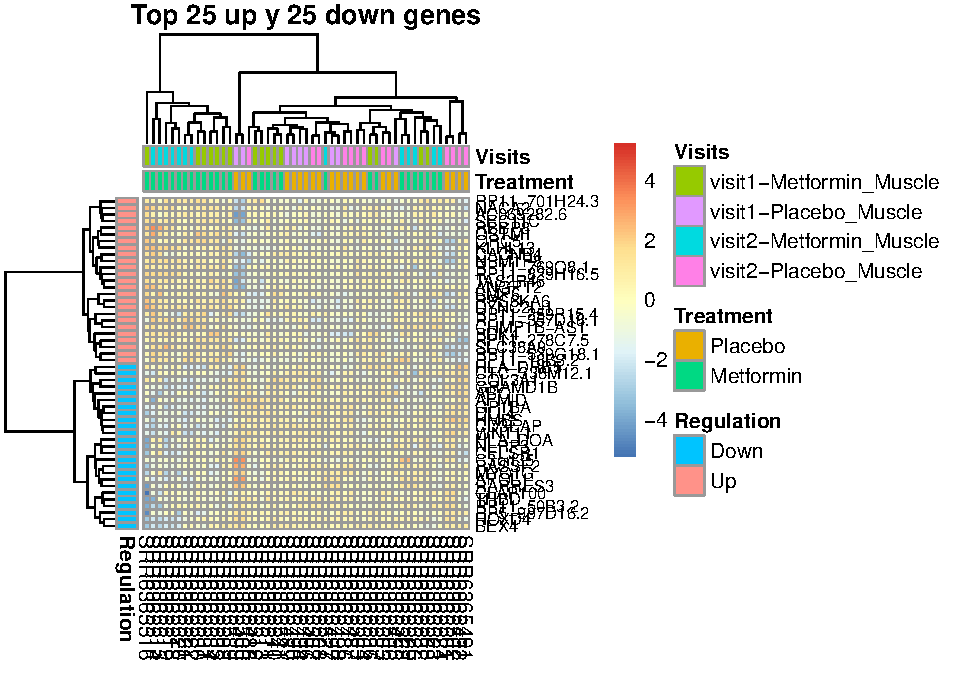
\includegraphics[keepaspectratio]{Proyecto_files/figure-latex/heatmap-1.pdf}}

Finalmente, el análisis de agrupamiento jerárquico (Heatmap) de los 50
genes con mayor varianza estadística reveló patrones de expresión
consistentes con la acción de la metformina, logrando distinguir bloques
de regulación positiva y negativa bien definidos. Si bien el dendrograma
de muestras reflejó la predominancia de la variabilidad interindividual
---confirmando los hallazgos del análisis de partición de varianza---,
los genes seleccionados mostraron una respuesta coordinada al
tratamiento. Marcadores como PDK4, AFMID y THBD exhibieron perfiles de
expresión contrastantes entre condiciones, sugiriendo que la metformina
induce una reprogramación metabólica específica en el músculo
esquelético que trasciende el ruido biológico basal de los sujetos.

\paragraph{Análisis de varianza para los genes más
significativos}\label{anuxe1lisis-de-varianza-para-los-genes-muxe1s-significativos}

\begin{Shaded}
\begin{Highlighting}[]
\CommentTok{\# Filtrar los genes up y down}
\NormalTok{vp\_up }\OtherTok{\textless{}{-}}\NormalTok{ vp[}\FunctionTok{rownames}\NormalTok{(vp) }\SpecialCharTok{\%in\%} \FunctionTok{rownames}\NormalTok{(top\_up), ]}
\NormalTok{vp\_down }\OtherTok{\textless{}{-}}\NormalTok{ vp[}\FunctionTok{rownames}\NormalTok{(vp) }\SpecialCharTok{\%in\%} \FunctionTok{rownames}\NormalTok{(top\_down), ]}

\NormalTok{geneNames\_up }\OtherTok{\textless{}{-}}\NormalTok{ top\_up}\SpecialCharTok{$}\NormalTok{SYMBOL[}\FunctionTok{match}\NormalTok{(}\FunctionTok{rownames}\NormalTok{(vp\_up), }\FunctionTok{rownames}\NormalTok{(top\_up))]}
\NormalTok{geneNames\_down }\OtherTok{\textless{}{-}}\NormalTok{ top\_down}\SpecialCharTok{$}\NormalTok{SYMBOL[}\FunctionTok{match}\NormalTok{(}\FunctionTok{rownames}\NormalTok{(vp\_down), }\FunctionTok{rownames}\NormalTok{(top\_down))]}

\CommentTok{\# Reemplazar rownames en vp\_up y vp\_down}
\FunctionTok{rownames}\NormalTok{(vp\_up) }\OtherTok{\textless{}{-}}\NormalTok{ geneNames\_up}
\FunctionTok{rownames}\NormalTok{(vp\_down) }\OtherTok{\textless{}{-}}\NormalTok{ geneNames\_down}

\NormalTok{effect }\OtherTok{\textless{}{-}} \StringTok{"group"}
\NormalTok{vp\_up\_sorted }\OtherTok{\textless{}{-}}\NormalTok{ vp\_up[}\FunctionTok{order}\NormalTok{(vp\_up[, effect], }\AttributeTok{decreasing =} \ConstantTok{TRUE}\NormalTok{), ]}
\NormalTok{vp\_down\_sorted }\OtherTok{\textless{}{-}}\NormalTok{ vp\_down[}\FunctionTok{order}\NormalTok{(vp\_down[, effect], }\AttributeTok{decreasing =} \ConstantTok{TRUE}\NormalTok{), ]}

\CommentTok{\# Graficar barras porcentuales}
\FunctionTok{plotPercentBars}\NormalTok{(vp\_up\_sorted) }\SpecialCharTok{+}
  \FunctionTok{ggtitle}\NormalTok{(}\StringTok{"Estructura de varianza {-} TOP Genes UP"}\NormalTok{)}
\end{Highlighting}
\end{Shaded}

\pandocbounded{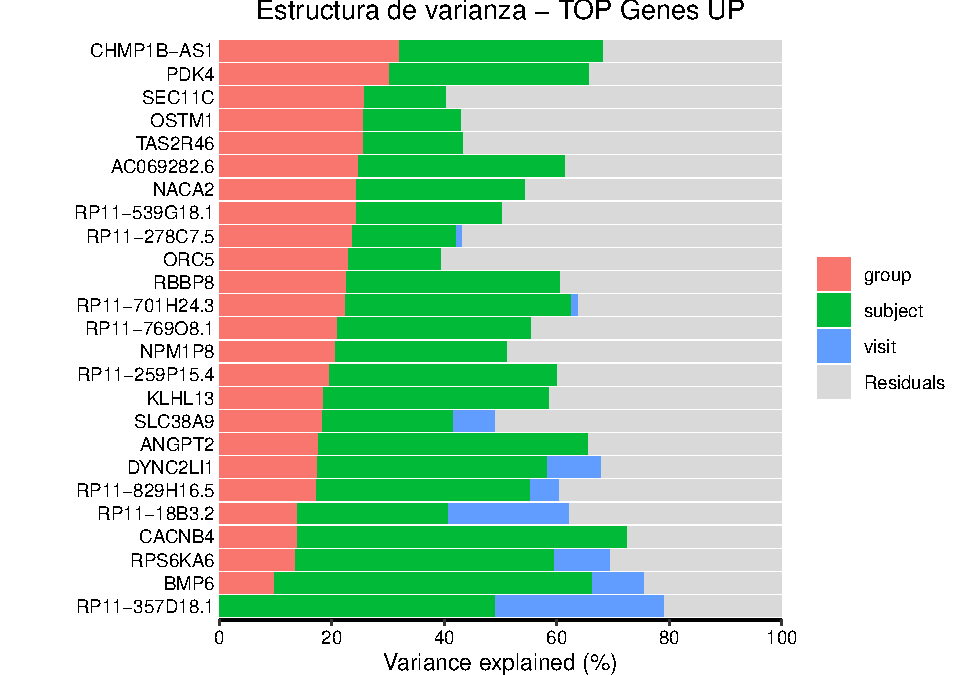
\includegraphics[keepaspectratio]{Proyecto_files/figure-latex/variance_top_genes_up-1.pdf}}

\begin{Shaded}
\begin{Highlighting}[]
\FunctionTok{plotVarPart}\NormalTok{(vp\_up) }\SpecialCharTok{+}
  \FunctionTok{ggtitle}\NormalTok{(}\StringTok{"Estructura de varianza {-} Genes UP"}\NormalTok{)}
\end{Highlighting}
\end{Shaded}

\pandocbounded{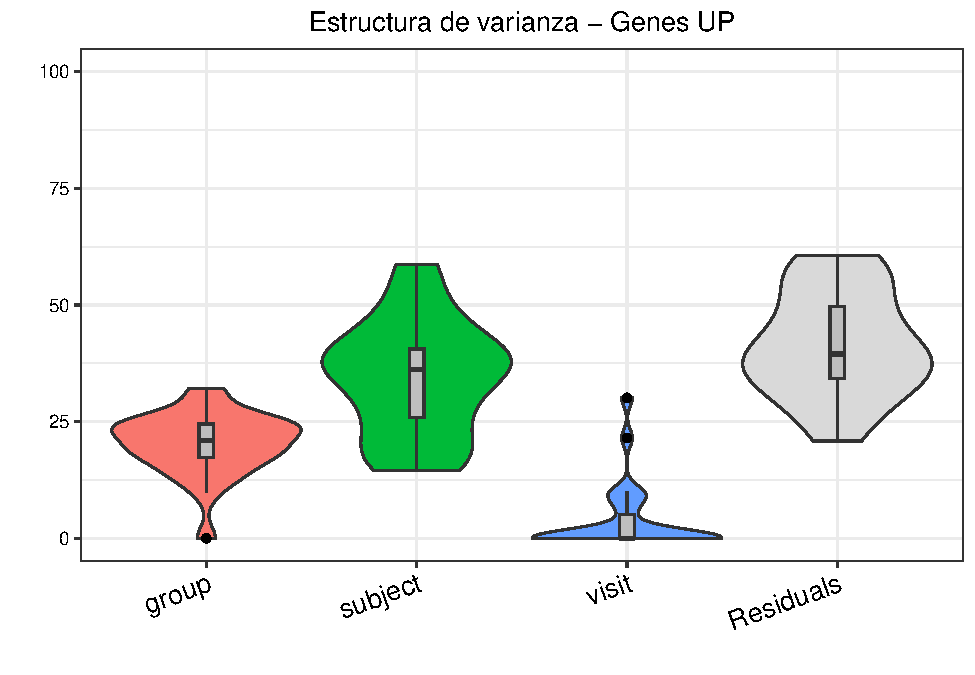
\includegraphics[keepaspectratio]{Proyecto_files/figure-latex/variance_top_genes_up-2.pdf}}

Al contrastar la estructura de varianza de los genes upregulated con la
tendencia global del transcriptoma, se observa un enriquecimiento
sustancial en la proporción de varianza explicada por el tratamiento
(group). Mientras que a nivel genómico el impacto de la metformina es
sutil, en el conjunto de genes UP este factor llega a explicar hasta el
30\% de la variabilidad total. Esta reducción proporcional de la
varianza residual, junto con la persistencia de un componente de sujeto
(subject) estable, sugiere que estos genes representan una respuesta
biológica robusta y consistente a través de la cohorte de adultos
mayores, permitiendo que la señal del fármaco trascienda la
heterogeneidad interindividual basal

\begin{Shaded}
\begin{Highlighting}[]
\CommentTok{\# Crear objetos}
\FunctionTok{plotPercentBars}\NormalTok{(vp\_down\_sorted) }\SpecialCharTok{+}
  \FunctionTok{ggtitle}\NormalTok{(}\StringTok{"Estructura de varianza {-} TOP Genes DOWN"}\NormalTok{)}
\end{Highlighting}
\end{Shaded}

\pandocbounded{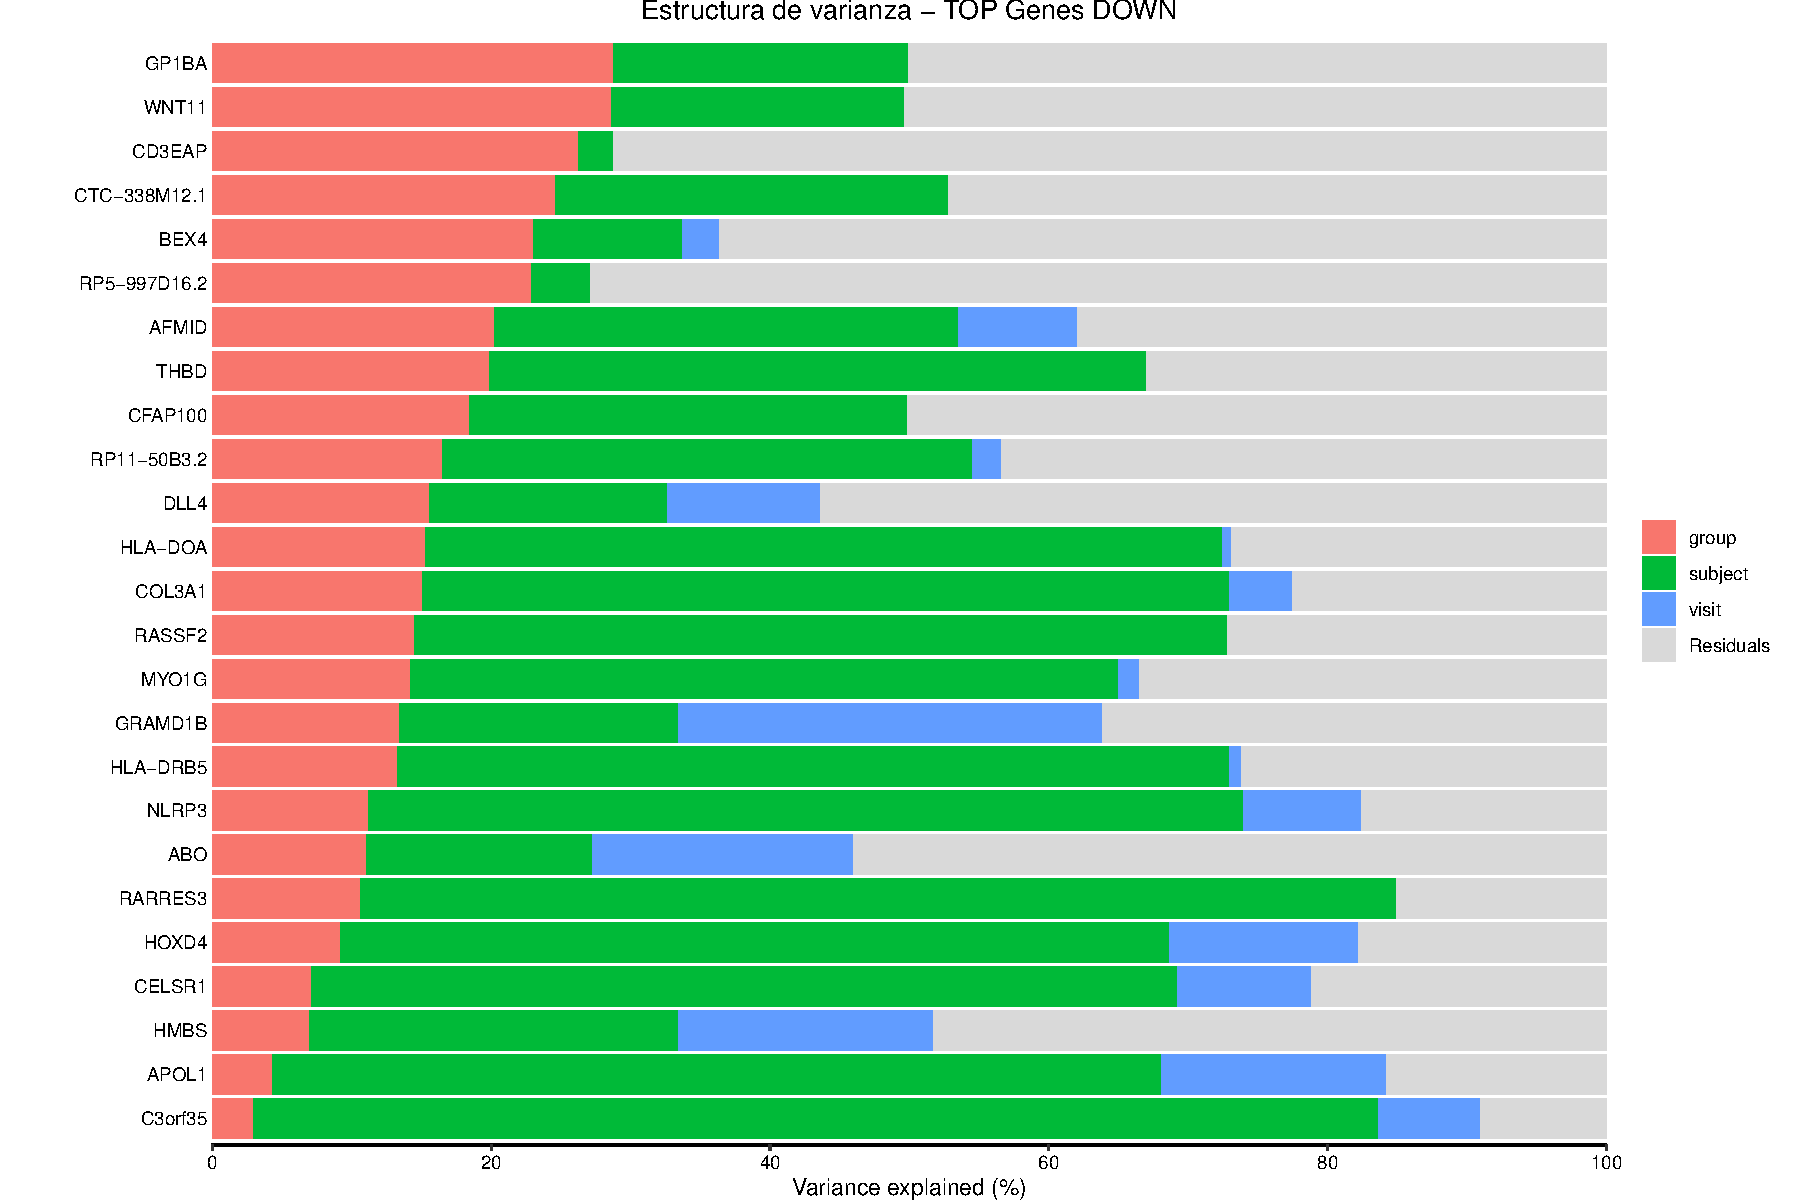
\includegraphics[keepaspectratio]{Proyecto_files/figure-latex/variance_top_genes_down-1.pdf}}

\begin{Shaded}
\begin{Highlighting}[]
\FunctionTok{plotVarPart}\NormalTok{(vp\_down) }\SpecialCharTok{+}
  \FunctionTok{ggtitle}\NormalTok{(}\StringTok{"Estructura de varianza {-} Genes DOWN"}\NormalTok{)}
\end{Highlighting}
\end{Shaded}

\pandocbounded{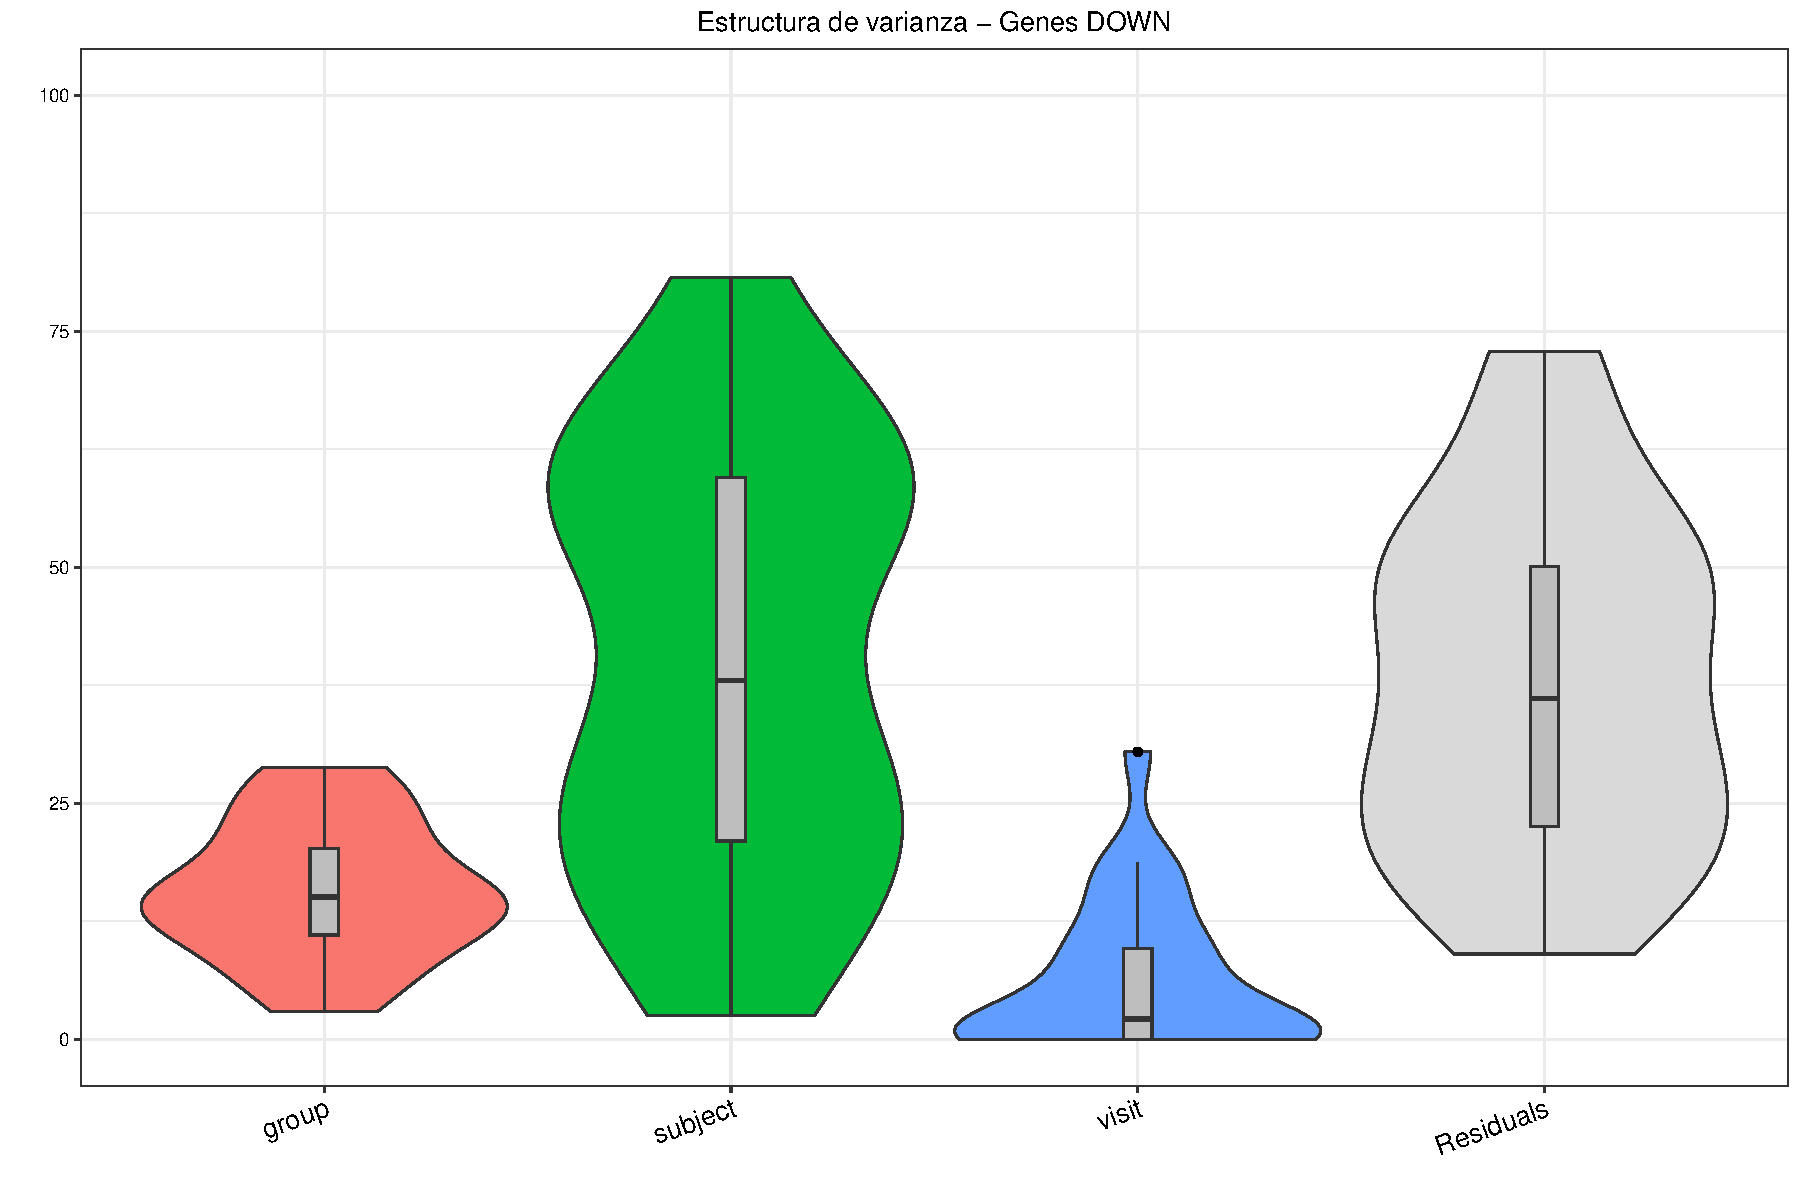
\includegraphics[keepaspectratio]{Proyecto_files/figure-latex/variance_top_genes_down-2.pdf}}

El análisis de la estructura de varianza para los genes con regulación
negativa (DOWN) ratificó la eficacia del modelo para aislar la señal del
tratamiento frente a la heterogeneidad biológica. Se observó que el
factor group explica una proporción sustancial de la variabilidad
(mediana \textasciitilde18\%), un incremento drástico frente al nivel
genómico basal. Notablemente, el componente subject mostró una
influencia predominante en este conjunto, sugiriendo que la magnitud de
la inhibición génica inducida por la metformina está íntimamente ligada
al perfil individual de cada adulto mayor. La marcada contracción de la
varianza residual en estos genes valida que los cambios identificados en
vías de inflamación y remodelado de la matriz extracelular son
estadísticamente robustos y representan una respuesta farmacológica
genuina.

\paragraph{MDS}\label{mds}

\begin{Shaded}
\begin{Highlighting}[]
\CommentTok{\# Seleccionar los genes de}
\NormalTok{genes\_sel }\OtherTok{\textless{}{-}} \FunctionTok{c}\NormalTok{(}\FunctionTok{rownames}\NormalTok{(top\_up), }\FunctionTok{rownames}\NormalTok{(top\_down))}
\NormalTok{expr\_sel }\OtherTok{\textless{}{-}}\NormalTok{ vobj}\SpecialCharTok{$}\NormalTok{E[genes\_sel, ]}

\FunctionTok{plotMDS}\NormalTok{(expr\_sel, }
        \AttributeTok{col =}\NormalTok{ colores[}\FunctionTok{as.numeric}\NormalTok{(meta}\SpecialCharTok{$}\NormalTok{group)],}
        \AttributeTok{pch =} \DecValTok{16}\NormalTok{,}
        \AttributeTok{cex =} \FloatTok{1.5}\NormalTok{,}
        \AttributeTok{main =} \StringTok{"MDS por tratamiento"}\NormalTok{,}
        \AttributeTok{xlab =} \StringTok{"Dimensión 1"}\NormalTok{,}
        \AttributeTok{ylab =} \StringTok{"Dimensión 2"}\NormalTok{)}

\CommentTok{\# Añadir leyenda mejorada}
\FunctionTok{legend}\NormalTok{(}\StringTok{"bottomleft"}\NormalTok{, }
       \AttributeTok{legend =} \FunctionTok{levels}\NormalTok{(meta}\SpecialCharTok{$}\NormalTok{group),}
       \AttributeTok{col =}\NormalTok{ colores[}\DecValTok{1}\SpecialCharTok{:}\FunctionTok{length}\NormalTok{(}\FunctionTok{levels}\NormalTok{(meta}\SpecialCharTok{$}\NormalTok{group))], }
       \AttributeTok{pch =} \DecValTok{16}\NormalTok{,}
       \AttributeTok{cex =} \FloatTok{0.8}\NormalTok{,}
       \AttributeTok{title =} \StringTok{"Tratamiento"}\NormalTok{,}
       \AttributeTok{bty =} \StringTok{"o"}\NormalTok{,           }\CommentTok{\# Con borde}
       \AttributeTok{bg =} \StringTok{"white"}\NormalTok{,        }\CommentTok{\# Fondo blanco}
       \AttributeTok{box.lwd =} \DecValTok{1}\NormalTok{)         }\CommentTok{\# Grosor del borde}
\end{Highlighting}
\end{Shaded}

\pandocbounded{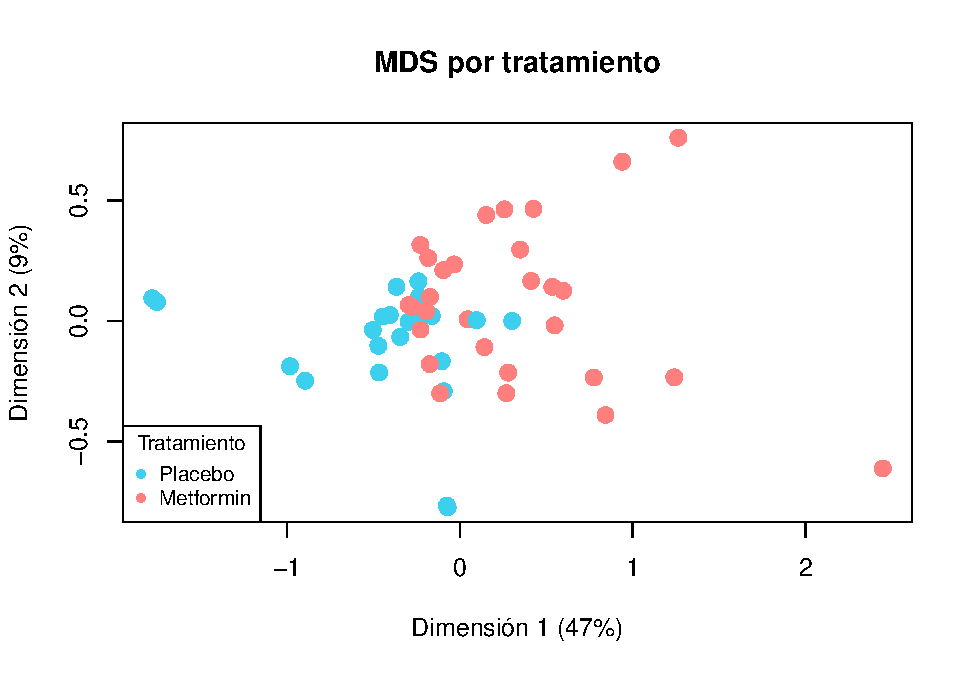
\includegraphics[keepaspectratio]{Proyecto_files/figure-latex/MDS_top_genes-1.pdf}}

La eficacia de la firma transcriptómica identificada se confirmó
mediante un análisis de escalamiento multidimensional (MDS) restringido
a los genes diferencialmente expresados. A diferencia del análisis
global, este modelo logró explicar el 57\% de la varianza total, con un
45\% concentrado en la primera dimensión, la cual separa de manera
efectiva las muestras tratadas con metformina de aquellas que recibieron
placebo. Este incremento sustancial en la varianza explicada demuestra
que, si bien la variabilidad interindividual es elevada, la metformina
induce cambios coordinados y consistentes en un conjunto específico de
genes metabólicos y estructurales, permitiendo una clara distinción
molecular entre las condiciones experimentales.

\subsubsection{Interpretación de
resultados}\label{interpretaciuxf3n-de-resultados}

\paragraph{GENES UPREGULATED}\label{genes-upregulated}

\begin{longtable}[]{@{}
  >{\raggedright\arraybackslash}p{(\linewidth - 4\tabcolsep) * \real{0.2083}}
  >{\raggedright\arraybackslash}p{(\linewidth - 4\tabcolsep) * \real{0.4167}}
  >{\raggedright\arraybackslash}p{(\linewidth - 4\tabcolsep) * \real{0.3750}}@{}}
\toprule\noalign{}
\begin{minipage}[b]{\linewidth}\raggedright
Gen
\end{minipage} & \begin{minipage}[b]{\linewidth}\raggedright
Producto
\end{minipage} & \begin{minipage}[b]{\linewidth}\raggedright
Función
\end{minipage} \\
\midrule\noalign{}
\endhead
\bottomrule\noalign{}
\endlastfoot
CHMP1B-AS1 & lncRNA antisense de CHMP1B & Regulación del gen CHMP1B,
posible modulación del tráfico endosómico, degradación de proteínas,
secreción de vesículas; potencial impacto en proliferación o
apoptosis \\
PDK4 & Piruvato deshidrogenasa quinasa 4 (enzima) & Fosforila e inhibe
el complejo piruvato deshidrogenasa (PDH), reduciendo la conversión de
piruvato a acetil-CoA; promueve el metabolismo de ácidos grasos sobre
glucosa. Mecanismo adaptativo de flexibilidad metabólica \\
DYNC2LI1 & Dynein Cytoplasmic 2 Light Intermediate Chain 1 (proteína,
subunidad ligera-intermedia de dineína 2) & Parte del complejo dineína 2
que participa en transporte retrógrado intraflagelar (IFT), moviendo
proteínas desde el extremo distal del cilio hacia la base. Podría
mejorar el transporte de receptores y señalización celular dependiente
de cilios, contribuyendo a la adaptación metabólica a metformina \\
RBBP8 & Retinoblastoma Binding Protein 8 (proteína, también llamada
CtIP) & Participa en reparación de ADN por recombinación homóloga,
resectando extremos de ADN en daños de doble cadena; también regula
progresión del ciclo celular en fase S/G2 \\
RPS6KA6 & Ribosomal Protein S6 Kinase A6 (RSK4, serina/treonina quinasa)
& Quinasa dependiente de MAPK, regula proliferación, diferenciación,
supervivencia celular, y puede inhibir el crecimiento celular; también
se ha vinculado con regulación de metabolismo energético \\
NACA2 & Nascent Polypeptide-Associated Complex Subunit Alpha 2 & Se une
a polipéptidos nacientes que no son secretorios mientras emergen del
ribosoma, evitando su destino inapropiado al ER. Bloquea la interacción
con la Signal Recognition Particle (SRP) y reduce la afinidad de los
ribosomas por sitios de translocación en la membrana del ER (M sites).
Previene agregación y asegura el correcto plegamiento y destino de
proteínas \\
ANGPT2 & Angiopoietin 2 (proteína secretada) & Ligando de los receptores
Tie2 en células endoteliales. Regula angiogénesis, remodelación vascular
y permeabilidad endotelial. Puede antagonizar ANGPT1-Tie2 para promover
desestabilización vascular y favorecer remodelado bajo estrés o
crecimiento \\
BMP6 & Bone Morphogenetic Protein 6 (proteína secretada, factor de
crecimiento TGF-β) & Regula diferenciación ósea y adipogénica,
metabolismo del hierro, angiogénesis y homeostasis celular; activa vías
SMAD dependientes \\
OSTM1 & Osteopetrosis Associated Transmembrane Protein 1 & Subunidad
reguladora de la ClC-7 necesaria para acidificación lisosomal y función
de osteoclastos; participa en homeostasis lisosomal, degradación de
proteínas y transporte de iones \\
SEC11C & Signal Peptidase Complex Subunit SEC11C & Subunidad del
complejo peptidasa de señal, que corta péptidos señal de proteínas
nacientes durante su translocación al retículo endoplásmico (ER);
esencial para maduración de proteínas secretadas \\
TAS2R46 & Taste receptor type 2 member 46 (receptor GPCR) & Receptor
acoplado a proteína G (GPCR) sensible a compuestos amargos. Participa en
señalización intracelular, incluyendo rutas de calcio y cAMP; se expresa
también fuera de la lengua, en células metabólicas y endoteliales \\
SLC38A9 & Solute Carrier Family 38 Member 9 (transceptor de aminoácidos,
transportador de arginina/lisina) & Actúa como sensor y transportador de
aminoácidos en lisosomas, regulando la vía mTORC1; permite que el
complejo Rag GTPasa detecte nutrientes y ajuste el crecimiento y
metabolismo \\
\end{longtable}

La firma molecular identificada en este estudio posiciona a la
metformina como un agente de resiliencia metabólica en el músculo
esquelético del adulto mayor. Un hallazgo central es la regulación
positiva de PDK4, que en conjunto con el sensor de aminoácidos lisosomal
SLC38A9, señala una restauración de la flexibilidad metabólica; la
capacidad de alternar eficientemente entre sustratos energéticos es una
facultad que declina con la edad y cuya pérdida subyace a la fragilidad
muscular. Esta reprogramación se complementa con la modulación de
quinasas y reguladores del ciclo celular como RPS6KA6 (RSK4) y RBBP8,
sugiriendo una optimización de las vías de supervivencia y reparación
del ADN frente al daño acumulado por el envejecimiento.

Particularmente relevante para el contexto geriátrico es el
fortalecimiento de los mecanismos de proteostasis y control de calidad
celular. La sobreexpresión de genes como NACA2, SEC11C y OSTM1 indica
una mejora en la fidelidad de la síntesis proteica y en la eficiencia de
la degradación lisosomal. Estos procesos son críticos, ya que la
acumulación de proteínas mal plegadas y la disfunción autofágica son
motores primarios de la sarcopenia. Asimismo, la identificación de
CHMP1B-AS1 y DYNC2LI1 apunta a una regulación sofisticada del tráfico
vesicular y la señalización mediada por cilios, mecanismos emergentes en
la adaptación metabólica celular.

Finalmente, la regulación de factores secretados y de señalización
intercelular, como ANGPT2, BMP6 y el receptor extra-gustativo TAS2R46,
sugiere una mejora en el microambiente tisular que abarca desde la
remodelación vascular hasta la homeostasis del hierro y la comunicación
paracrina. En conjunto, estos resultados demuestran que el impacto de la
metformina trasciende el control glucémico convencional, actuando como
un geroprotector integral capaz de intervenir en los pilares del
mantenimiento celular necesarios para preservar la funcionalidad física
y la autonomía en la vejez.

\subsubsection{GENES DOWNREGULATED}\label{genes-downregulated}

\begin{longtable}[]{@{}
  >{\raggedright\arraybackslash}p{(\linewidth - 4\tabcolsep) * \real{0.2083}}
  >{\raggedright\arraybackslash}p{(\linewidth - 4\tabcolsep) * \real{0.4167}}
  >{\raggedright\arraybackslash}p{(\linewidth - 4\tabcolsep) * \real{0.3750}}@{}}
\toprule\noalign{}
\begin{minipage}[b]{\linewidth}\raggedright
Gen
\end{minipage} & \begin{minipage}[b]{\linewidth}\raggedright
Producto
\end{minipage} & \begin{minipage}[b]{\linewidth}\raggedright
Función
\end{minipage} \\
\midrule\noalign{}
\endhead
\bottomrule\noalign{}
\endlastfoot
GRAMD1B & GRAM domain-containing protein 1B & Proteína de membrana que
regula transporte de colesterol y lípidos entre retículo endoplásmico y
membrana plasmática, manteniendo homeostasis lipídica y señalización.
Podría significar un ajuste del metabolismo lipídico, disminuyendo
transporte de lípidos hacia la membrana y favoreciendo rutas de
catabolismo de energía \\
WNT11 & Wnt family member 11 (proteína secretada, señalización no
canónica) & Señalización no canónica Wnt que regula morfogénesis,
polaridad celular, migración y remodelado citosquelético; contribuye a
diferenciación celular y desarrollo vascular.Ajuste selectivo del
remodelado celular, reduciendo migración y reorganización activa del
citosqueleto, \\
GP1BA & Glycoprotein Ib platelet subunit alpha & Subunidad alfa del
receptor GP Ib-IX-V; participa en adhesión plaquetaria, señalización y
hemostasia, interactuando con factor de von Willebrand \\
COL3A1 & Collagen type III alpha 1 chain (proteína estructural ECM) &
Componente de la matriz extracelular, aporta elasticidad y soporte
estructural a vasos sanguíneos, piel y tejido conectivo; participa en
remodelado tisular y señalización mecánica. La disminución tras
metformina podría reflejar reducción del remodelado ECM activo \\
THBD & Thrombomodulin (proteína transmembrana endotelial) & Receptor
transmembrana que se une a trombina, activando proteína C
anticoagulante; regula coagulación, inflamación y homeostasis vascular.
modulación del microambiente vascular y reducción de estrés hemostático
en respuesta a cambios metabólicos \\
RARRES3 & Retinoic acid receptor responder protein 3 & Proteína inducida
por retinoides que regula diferenciación celular, señalización
antiproliferativa y homeostasis de membranas lipídicas; puede tener
efectos en estrés celular y control de crecimiento. Refleja reducción de
señales de diferenciación o estrés celular no prioritario \\
AFMID & Arylformamidase & Enzima que cataliza un paso en la vía de
degradación del triptófano hacia la niacinamida y NAD⁺, modulando
metabolismo energético y estrés oxidativo \\
NLRP3 & NLR family pyrin domain containing 3 (inflammasoma) & Sensor
citosólico que forma el inflammasoma NLRP3, activando caspasa-1,
maduración de IL-1β/IL-18 y respuesta inflamatoria \\
HLA-DOA & Major histocompatibility complex, class II, DO alpha &
Subunidad alfa de HLA-DO, que regula la presentación de antígenos por
HLA clase II, modulando la carga de péptidos en células presentadoras de
antígeno. Rducción de activación inmune adaptativa local \\
RASSF2 & Ras association domain family member 2 & Proteína supresora de
tumores que regula Ras-MAPK, apoptosis y ciclo celular; modula respuesta
a estrés y control de proliferación \\
HOXD4 & Homeobox D4 & Factor de transcripción de la familia HOX, regula
desarrollo, diferenciación celular y expresión génica específica de
tejidos \\
APOL1 & Apolipoprotein L1 & Proteína implicada en transporte de lípidos,
defensa contra patógenos y regulación de estrés oxidativo en células \\
CD3EAP & CD3e molecule associated protein & Participa en transcripción
ribosomal, regulación de proliferación y control del ciclo celular;
asociado a la síntesis de ARN ribosomal y ensamblaje ribosomal \\
\end{longtable}

La respuesta de inhibición génica observada tras el tratamiento con
metformina revela una desactivación coordinada de procesos patológicos
intrínsecos al envejecimiento muscular. Esta «firma de apagado» se
manifiesta, en primera instancia, a través de la atenuación del
inflammaging y una profunda reprogramación inmune; la regulación a la
baja de sensores críticos del inflammasoma, como NLRP3, y de moléculas
de presentación de antígenos, como HLA-DOA, sugiere una pacificación del
microambiente inmunológico que protege al tejido del daño colateral
provocado por una respuesta inmune local crónicamente sobreactivada.
Complementariamente, se identifica un control estricto sobre la dinámica
de la matriz extracelular (ECM), evidenciado por la reducción de
componentes estructurales como COL3A1 y mediadores de remodelado
citosquelético como WNT11. Dado que el envejecimiento muscular se asocia
con un proceso de fibro-sustitución que compromete la potencia y
elasticidad, la disminución de estos genes sugiere que la metformina
actúa frenando la expansión de la red fibrótica y preservando la
integridad arquitectónica del tejido.

Asimismo, la inhibición de reguladores del transporte lipídico,
representados por GRAMD1B y APOL1, apunta a una recalibración del
metabolismo de lípidos y de la homeostasis de membranas. Este ajuste es
fundamental en adultos mayores para mejorar la fluidez de la membrana
plasmática y optimizar la señalización de receptores metabólicos, como
el de la insulina, frecuentemente entorpecida por la acumulación
lipídica ectópica. Finalmente, el descenso en la expresión de factores
de transcripción y reguladores del ciclo celular, tales como HOXD4 y
RASSF2, sugiere una transición hacia un estado de «quietud metabólica» y
ahorro energético. Al desactivar programas de diferenciación y
proliferación potencialmente ineficientes en un contexto de senescencia,
el fármaco parece redirigir los recursos celulares hacia mecanismos de
mantenimiento, reparación y resiliencia proteica. En conjunto, esta
respuesta negativa no representa una pérdida de función, sino una
intervención geroprotectora dual que desactiva las rutas de inflamación
y rigidez estructural para restaurar un perfil molecular más saludable y
funcional.

\subsection{CONCLUSIÓN}\label{conclusiuxf3n}

El presente estudio demuestra que el tratamiento con metformina en
adultos mayores induce una reprogramación transcriptómica integral en el
músculo esquelético, orientada hacia la restauración de la homeostasis
celular y la resiliencia metabólica. Mediante la aplicación del modelo
de efectos mixtos dream, fue posible discernir una firma molecular
robusta a pesar de la elevada heterogeneidad interindividual propia de
la población geriátrica. El análisis de la estructura de varianza
confirmó la solidez de estos hallazgos: mientras que a nivel genómico
global el efecto del tratamiento es sutil, en los genes identificados el
factor group (metformina vs.~placebo) logró explicar entre el 15\% y el
30\% de la variabilidad total, superando significativamente al ruido
residual.

Esta respuesta se caracteriza por una acción dual geroprotectora
claramente diferenciada en su arquitectura de varianza. Por un lado, la
activación de mecanismos críticos de proteostasis, flexibilidad
metabólica y reparación celular ---liderada por genes como PDK4 y
NACA2--- mostró una respuesta altamente consistente entre sujetos. Por
otro lado, se observó una desactivación coordinada de procesos
deletéreos como la inflamación crónica (inflammaging) y la fibrosis
tisular ---mediada por la represión de NLRP3 y COL3A1---, cuya magnitud
de inhibición estuvo íntimamente ligada al perfil basal de cada
individuo, evidenciando una modulación personalizada del microambiente
muscular.

En conjunto, estos hallazgos posicionan a la metformina no solo como un
agente hipoglucemiante, sino como una intervención terapéutica capaz de
mitigar múltiples pilares del envejecimiento biológico. Al demostrar una
capacidad única para ``limpiar'' la señal del fármaco frente al ruido
del envejecimiento, este estudio ofrece una base molecular sólida para
el uso de la metformina en la preservación de la función muscular y la
prevención de la fragilidad en la vejez.

\section{Referencias}\label{referencias}

\end{document}
